\chapter{Resultados}
\label{cap:resultados}

%Neste capítulo serão discutidos os resultados da análise dos dados coletados, bem como resultados referentes ao modelo de regressão criado para utilizar os dados como um auxílio para desenvolvimento de projetos futuros.
%TODO criar explicação geral para o capítulo
%TODO relacionar resultados das métricas a padrões de projeto

\section{Análise preliminar}

Com os dados coletados e devidamente preparados, várias conclusões podem ser tiradas dos valores das métricas e sua evolução ao longo do tempo. Esta seção é focada na análise subjetiva dos dados, tentando explicar seu comportamento com relação às características do sistema, compará-los a outros estudos, e até mesmo comparar com dados de métricas em aplicativos, utilizando os próprios aplicativos do sistema como base de comparação.

Embora seja relevante comentar as diferenciações entre as linguagens e seus paradigmas para algumas métricas,  não há necessidade de separação entre os valores para linguagem C, procedural, e linguagens Java/C++, orientadas a objetos, uma vez que, dadas as proporções das mesmas apresentadas nos dados, não há relevância estatística para tal. Entretanto em algumas métricas algumas observações teóricas possam ser ressaltadas, embora, mais uma vez, não haja implicação substancial no resultados gerais apresentados.

\subsection{Average Method Lines Of Code}

A primeira observação que deve ser feita quando analisando LOC nesse contexto é a diferenciação das linguagens. Embora um módulo em C seja mapeado para uma classe, arquivos fonte em C tendem a ser maiores que uma classe em Java, por exemplo, devido aos diferentes paradigmas que essas linguagem utilizam. Arquivos em C++ e Java também podem ter valores bem distintos para a mesma funcionalidade devido ao número de bibliotecas padrões que a linguagem apresenta e a natureza da própria sintaxe da linguagem. Dessa forma, comparações dessa métrica devem ser feitas somente dentro da mesma linguagem. 
%Neste trabalho não serão feitas comparações diretas dos valores desta métrica, então ela será utilizada principalmente para relativização da comparação de outras métricas, quando aplicável, uma vez que os valores de algumas delas podem ser relacionados a esta. 

A métrica LOC por si só não será discutida aqui, pois seu valor é mais relativo e deve ser comparado com outras métricas para ter significado mais completo. Uma classe com valor alto de LOC pode ter um baixo valor de AMLOC e valor maior para NOM, ainda mantendo um valor aceitável de LCOM. Em suma, a análise de outras métricas abrange as explicações relacionadas a métrica LOC e também a NOM, então essas métricas de tamanho não serão explanadas em separado, mas juntamente com a explicação de outras métricas.

Valores baixos de AMLOC são sempre preferíveis pois métodos mais enxutos tem menor responsabilidade, portanto estão mais sujeitos a reuso, e também são mais fáceis de se ler e se modificar. Entretanto essa métrica é preciso ser analisada em conjunto com outras métricas, como LCOM e RFC. Uma classe com muitos métodos privados pequenos tende a ter um valor maior de RFC, o que não implica que esteja mal projetada, desde que os métodos ali presentes estejam bem posicionados segundo o padrão de projeto OO especialista da informação, mantendo por consequencia um baixo valor de LCOM. Como referência geral de resultados para AMLOC, quanto menor o valor, melhor o resultado.

\begin{table}[!htb]
\scalefont{.7}
\documentclass[a4paper]{article}
\usepackage[T1]{fontenc}
\usepackage[latin1]{inputenc}
\begin{document}
\begin{tabular}{|l|l|l|l|l|l|l|l|l|l|l|l|}
\hline
version&min&1\%&5\%&10\%&25\%&50\%&75\%&90\%&95\%&99\%&max\\
\hline
android-1.6\_r1.2&0&0&0&0&2.33333333333333&5.57142857142857&11.5&21.5&30&65.8742857142858&312\\
\hline
android-1.6\_r1.5&0&0&0&0&2.33333333333333&5.57142857142857&11.5&21.5&30&65.8742857142858&312\\
\hline
android-2.0\_r1&0&0&0&0&2&5.55555555555556&11.5&21.8461538461538&30.1916666666666&67.8124999999999&390.5\\
\hline
android-2.1\_r2.1p2&0&0&0&0&2&5.625&11.5&21.8571428571429&30.3366666666666&68.4017499999999&395\\
\hline
android-2.2\_r1&0&0&0&0&1.75892857142857&5.8&12.8&26.5&44.2135714285714&156.66&1034\\
\hline
android-2.2.3\_r2&0&0&0&0&1.76587301587301&5.81666666666666&12.8214285714286&26.5&44.1664285714285&156.62&1034\\
\hline
android-2.3\_r1&0&0&0&0&1&5.8&13.6&30.1787878787879&55.3636363636363&164.773333333334&1034\\
\hline
android-2.3.7\_r1&0&0&0&0&1&5.83333333333333&13.7064950980392&30&54.0590277777778&163.397272727272&1034\\
\hline
android-4.0.1\_r1&0&0&0&0&1&5.85714285714286&14&31&54.3731481481482&162.418181818181&1034\\
\hline
android-4.0.4\_r2.1&0&0&0&0&1&5.85714285714286&14&31&53.9791666666667&162&1034\\
\hline
\end{tabular}
\end{document}

\scalefont{.7}
\caption{Percentis para a métrica \textit{Average Method Lines of Code} no Android}
\label{tab:amloc_android}
\end{table}

\begin{figure}[!htb]
\centering
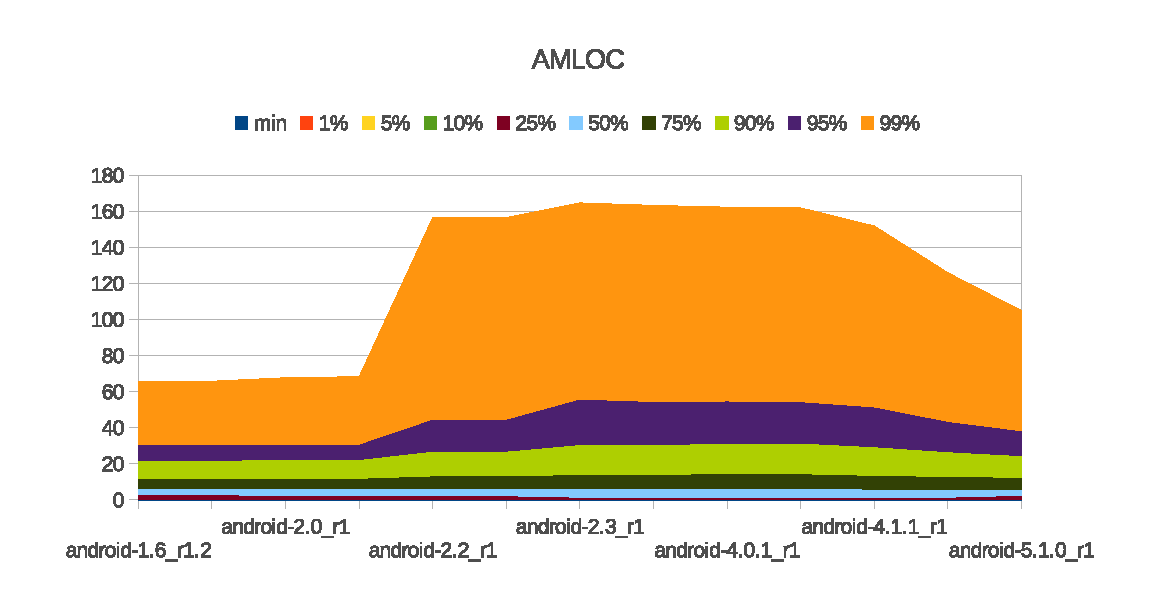
\includegraphics [keepaspectratio=true,scale=0.85]{figuras/graphs/amloc_android.eps}
\caption{Evolução da métrica AMLOC ao longo das versões da API}
\label{fig:amloc_android}
\end{figure}

A Tabela~\ref{tab:amloc_android} apresenta os valores para a métrica AMLOC nas versões do Android analisadas. É facilmente perceptível que a média de linhas de código por método não teve variação relevante. Em todas as versões analisadas, os valores muito frequentes, isto é, percentil 75, são métodos com até 14 linhas de código, enquanto de 14 a 30 aparecem como frequentes, e 31 a 55 pouco frequentes. A Figura~\ref{fig:amloc_android} apresenta a evolução da métrica AMLOC com a API, onde é possível ver uma variação muito pequena de valores para os percentis 75 e 90. O percentil 99 demonstra uma variação maior, mas ele representa dados não frequentes na análise.

Esses são valores que estão de acordo com os apresentados em \citeonline{meirelles2013}, porém levemente menores para os percentis 75 e 90, com aproximadamente 3 linhas de código a menos por método. É possível perceber que os valores se mostraram bem semelhantes para o projeto Android, mesmo considerando o fato que este trabalho estuda apenas a API de desenvolvimento de aplicativos, essencialmente em Java e dentro do diretório ``\textit{frameworks}'' do AOSP, e \citeonline{meirelles2013} analiza todo o código fonte do sistema, que apresenta em sua totalidade uma maior proporção da linguagem C em relação as demais. Esses valores são subsídios para reafirmar que arquivos em C em geral, tem uma maior utilização de linhas de código do que arquivos em Java. \citeonline{oliveira2013} comenta que as diferenças entre as linguagems C/C++/Java para esta métrica não é significativa, uma vez que a sintaxe entre as 3 é bastante semelhante. Dada essa afirmação, podemos comparar os intervalos definidos por ele, chegando a conclusão de que os valores das métricas estão, para todas as versões, abaixo dos valores e regular para os percentis 75 e 90, o que é um bom resultado.

\begin{table}[!htb]
\scalefont{.7}
\begin{tabular}{|l|l|l|l|l|l|l|l|l|l|l|l|l|}
\hline
app&classes&min&1\%&5\%&10\%&25\%&50\%&75\%&90\%&95\%&99\%&max\\
\hline
Launcher2&161&0&0&1&1&3&6.33&10.78&16.9&24.38&48.36&57.5\\
\hline
Settings&722&0&0&0&0&3.63&8&15&21.47&28.5&49.4&80.42\\
\hline
Camera2&462&0&0&0&0&1&4.5&9.85&16.09&21.5&38.28&66.67\\
\hline
Bluetooth&239&0&0&0&2.83&6.02&10.79&22.16&39.86&59.84&111.11&221\\
\hline
QuickSearchBox&196&0&0&1&1&3&4.39&6.17&10.53&13.15&22.28&32\\
\hline
Calculator&10&1&1&1&1&6.67&8.92&13.33&23.26&27.38&30.68&31.5\\
\hline
Terminal&17&0&0.15&0.75&1.85&3.09&8.12&15.29&20.92&29.38&48.27&53\\
\hline
PackageInstaller&19&0&0.68&3.4&4&4.63&6.59&16.98&18.9&22.89&31.45&33.59\\
\hline
Dialer&215&0&0&0&1&3&7&11.13&16.89&19.98&32.02&61.33\\
\hline
Browser&259&0&0&1&1&3.5&6.89&11&19&25.95&46.02&55.33\\
\hline
InCallUI&117&0&0&0&0&1&4.23&12&18.75&23.32&40.77&58\\
\hline
LegacyCamera&214&0&0&0&0.2&4&8.64&15.78&25.47&32.18&69.42&112.67\\
\hline
Gallery2&895&0&0&0&0&3&6&11.5&17.38&21.67&44.36&107\\
\hline
BasicSmsReceiver&5&8.67&8.83&9.47&10.27&12.67&16.33&18.75&18.9&18.95&18.99&19\\
\hline
UnifiedEmail&872&0&0&0&1&3&5&9.71&17&23.67&37.95&139.63\\
\hline
Launcher3&354&0&0&0&0&2.73&5.13&10.59&17.17&24.79&54.71&163.5\\
\hline
Music&75&0&0&0&1&4.1&9.51&16.89&21.76&28.0&48.32&90\\
\hline
Camera&253&0&0&0&1&3&7.42&13&22.37&31.45&72.23&112.67\\
\hline
Email&400&0&0&0&1&3.58&8&15.35&24.49&31.61&63.28&128\\
\hline
Nfc&178&0&0&0&1&3&9.64&18.5&31.63&38&42.48&70.5\\
\hline
Gallery&89&0&0.87&1&1&4&7.63&12.67&19.0&28.6&53.12&55\\
\hline
ContactsCommon&292&0&0&0&1&3.23&7.1&13&19&23.88&34.5&53.33\\
\hline
Contacts&265&0&0&0&1&3&6.45&11.5&18.61&23.72&63.53&86\\
\hline
DeskClock&121&0&0&0&1&5&9.16&15.26&24.02&27.3&30.71&40.13\\
\hline
HTMLViewer&4&5&5.12&5.6&6.2&8&11&14.5&16.6&17.3&17.86&18\\
\hline
Calendar&216&0&0&0&1&5&11.67&19.58&30.95&39.3&90&115.5\\
\hline
Exchange&135&0&0&0&1&4&10.01&17.31&28.41&34.65&44.41&51.25\\
\hline
\end{tabular}

\scalefont{.7}
\caption{Percentis para a métrica \textit{Average Method Lines of Code} nos aplicativos nativos}
\label{tab:amloc_apps}
\end{table}

Os valores apresentados na análise são relativamente baixos quando comparados com outros softwares livres, como demonstrado por \citeonline{meirelles2013}. Da mesma forma, quando olhamos os valores aplicativos do sistema, demonstrados na Tabela~\ref{tab:amloc_apps}, podemos perceber uma grande semelhança nos resultados. Embora alguns poucos aplicativos tenham valores mais elevados para essa métrica, pode-se perceber que os intervalos se mantém válidos para a grande maioria dos aplicativos. Esses valores de aplicativos foram retirados dos aplicativos nativos da ultima versão do sistema analisada (Lollipop 5.1.0), e continuam se mantendo semelhantes ao sistema, como o próprio acoplamento à API sugere.

Em linhas gerais, os aplicativos do sistema também se mantém dentro dos intervalos bom e regular definidos em \citeonline{oliveira2013}. Os valores para o percentil 95 também se encontram abaixo do valor regular, na maioria dos casos.

Em suma, os valores para os aplicativos se assemelham muito com os valores para as versões da API Android analisadas, levando então a conclusão de que os mesmos intervalos são válidos para as métricas em ambos os casos, embora se possa esperar valores menores em aplicativos, porem com uma maior variância. Essa variância se dá pelo diferente propósito de cada aplicativo, que utiliza pedaços variados do sistema e tem sua codificação adaptada para seu propósito.

Intervalos encontrados:

\begin{itemize}
\item Valores abaixo de 14 se mostraram muito frequentes para os aplicativos e para a API;
\item Enquanto no sistema os valores para o percentil 90 se encontram abaixo de 31, nos aplicativos eles alcançam em poucos casos, ficando em sua maioria abaixo de 25;
\item Valores acima de 31 são pouco frequentes em ambos os casos;
\end{itemize}

\subsection{Average Cyclomatic Complexity per Method}

Complexidade ciclomática nada mais é do que o número de caminhos que um software pode seguir dada uma execução qualquer. Na prática, cada condicional dentro do sistema incrementa o valor desta métrica em 1, uma vez que divide a execução em um caminho de execução se a expressão condicional for válida, ou um segundo caminho caso não seja. Complexidade ciclomática é calculada a nível de método, e o valor de ACCM para uma classe corresponde a média dos valores de complexidade ciclomática de cada um dos seus métodos.

\begin{figure}[!htb]
\centering
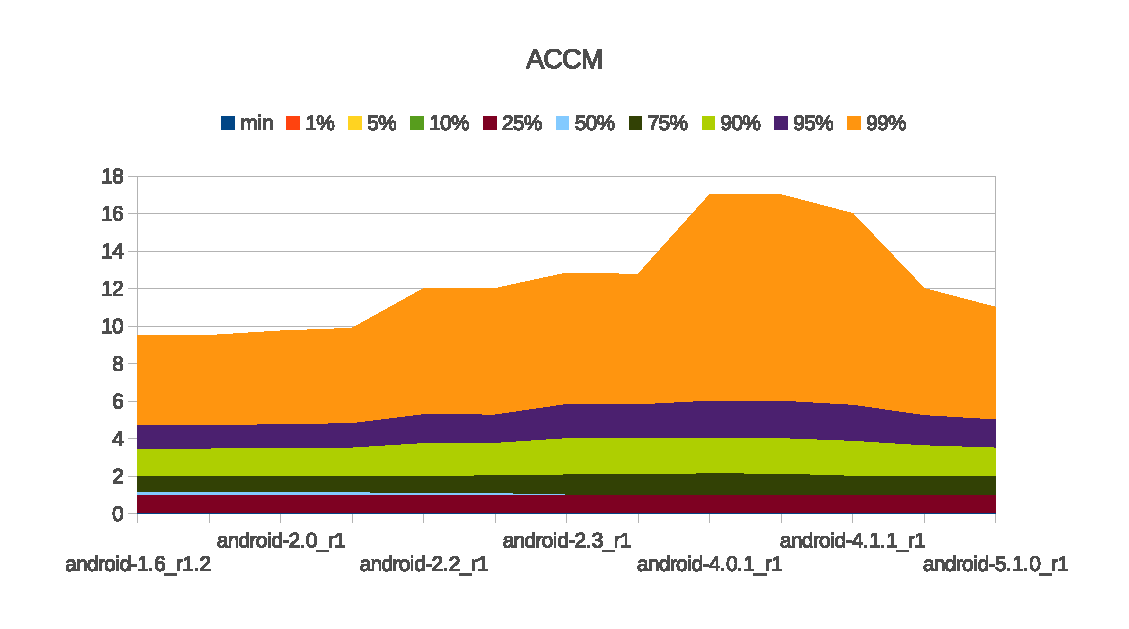
\includegraphics [keepaspectratio=true,scale=0.85]{figuras/graphs/accm_android.eps}
\caption{Evolução da métrica ACCM ao longo das versões da API}
\label{fig:accm_android}
\end{figure}

A interpretação do valor de complexidade ciclomática é relativamente simples: O valor 1 é o valor mínimo e ideal para se ter como resultado, pois significa que o software tem apenas uma forma de executar e será executado necessariamente daquela forma e naquela sequência. Como consequência disso, se tem um software que pode ser mais facilmente lido e modificado. A implicação dessa métrica é mais notada na atividade de testes do código fonte, pois além de dificultar a compreensão dos possíveis comportamentos de um pedaço de código, cada caminho adicional que pode ser seguido é um trecho diferenciado que deve ser testado. Isso quer dizer que o esforço de teste é diretamente proporcional ao resultado dessa métrica, pois para garantir o funcionamento correto do sistema, todos as possibilidades devem ser devidamente testadas. Em termos práticos, atingir uma cobertura de código de 100\% é uma tarefa árdua quando há um valor muito grande de complexidade ciclomática.

A Figura~\ref{fig:accm_android} apresenta a evolução dessa métrica com a evolução da API. Podemos perceber que essa métrica não teve uma variação grande ao longo das versões nos percentis 75, 90 e 95, e o pouco do valor que ganhou nas versões centrais do gráfico foi sendo novamente reduzido nas versões seguintes.

\begin{table}[!htb]
\scalefont{.7}
\begin{tabular}{|l|l|l|l|l|l|l|l|l|l|l|l|l|}
\hline
versão&classes&min&1\%&5\%&10\%&25\%&50\%&75\%&90\%&95\%&99\%&max\\
\hline
android-1.6\_r1.2&5745&0&0&0&0&1&1.11&2&3.45&4.69&9.5&55\\
\hline
android-1.6\_r1.5&5745&0&0&0&0&1&1.11&2&3.45&4.69&9.5&55\\
\hline
android-2.0\_r1&6331&0&0&0&0&1&1.11&2&3.5&4.75&9.74&59\\
\hline
android-2.1\_r2.1p2&6360&0&0&0&0&1&1.12&2&3.5&4.8&9.88&60\\
\hline
android-2.2\_r1&7352&0&0&0&0&1&1.07&2&3.74&5.28&12&99\\
\hline
android-2.2.3\_r2&7358&0&0&0&0&1&1.07&2.02&3.75&5.26&12&99\\
\hline
android-2.3\_r1&8093&0&0&0&0&1&1&2.07&4&5.82&12.83&99\\
\hline
android-2.3.7\_r1&8240&0&0&0&0&1&1&2.08&4&5.8&12.76&99\\
\hline
android-4.0.1\_r1&11709&0&0&0&0&1&1&2.13&4&6&17&94.33\\
\hline
android-4.0.4\_r2.1&11851&0&0&0&0&1&1&2.11&4&6&17&94.33\\
\hline
android-4.1.1\_r1&14115&0&0&0&0&1&1&2&3.86&5.78&16&99.4\\
\hline
android-4.3.1\_r1&15472&0&0&0&0&1&1&2&3.62&5.23&12&120.4\\
\hline
android-5.1.0\_r1&20129&0&0&0&0&1&1&2&3.5&5&11&158.6\\
\hline
\end{tabular}

\scalefont{.7}
\caption{Percentis para a métrica \textit{Average Cyclomatic Complexity per Method} no Android}
\label{tab:accm_android}
\end{table}

Inserida então no contexto de manutenção e testes, essa métrica é uma excelente candidata para ser constantemente monitorada ao longo da evolução do código fonte. Embora não tenha muita relação com outras métricas OO, ACCM tem uma relação óbvia do número de linhas de código de um método, pois um método com poucas linhas de código não tem possibilidade de ter um valor muito alto de complexidade ciclomática. De forma geral, métodos grandes ``abrem espaço'' para problemas de complexidade excessiva, como já comentado na seção anterior. Essa relação pode ser claramente vista na Tabela~\ref{tab:accm_android}. Nos valores do percentil 75, que correspondem a valores muito frequentes, as versões de 2.2.3 a 4.0.4 contém os únicos valores para o sistema onde essa métrica supera o número 2, e não por acaso são os valores com maior AMLOC nesse percentil como pode ser visto na Tabela~\ref{tab:amloc_android}. Essa relação direta também pode ser vista nos percentis 90 e 95, que representam valores frequentes e pouco requentes, respectivamente.

\begin{table}[!htb]
\scalefont{.7}
\documentclass[a4paper]{article}
\usepackage[T1]{fontenc}
\usepackage[latin1]{inputenc}
\begin{document}
\begin{tabular}{|l|l|l|l|l|l|l|l|l|l|l|l|}
\hline
app&min&1\%&5\%&10\%&25\%&50\%&75\%&90\%&95\%&99\%&max\\
\hline
Launcher2&0&0&1&1&1&1.4&2.09318181818182&3&3.61545454545454&8.67642857142855&11.8666666666667\\
\hline
Settings&0&0&0&0&1&1.57142857142857&2.5&3.66666666666667&4.42857142857143&8&17\\
\hline
Camera2&0&0&0&0&1&1&1.83333333333333&2.66666666666667&3.5&6&8.3\\
\hline
Bluetooth&0&0&0&1&1.33333333333333&2.19337979094077&4&7.95&10.3625&24.2866666666666&49\\
\hline
VoiceDialer&1&1&1&1&1.75&3.5&6.16666666666667&8.52&8.93999999999999&11.388&12\\
\hline
QuickSearchBox&0&0&1&1&1&1.03333333333333&1.66666666666667&2.47142857142857&3&4.67666666666667&5\\
\hline
Calculator&1&1&1&1&1.33333333333333&1.58333333333333&2.66666666666667&3.53333333333333&5.26666666666667&6.65333333333333&7\\
\hline
Mms&0&0&0&0&1&1.28571428571429&2.43650793650793&3.55555555555556&5.4125&10.2285714285714&16\\
\hline
ManagedProvisioning&1&1&1&1&1&2.16764705882353&2.98076923076923&3.24&3.575&5.26000000000001&6\\
\hline
SoundRecorder&1&1.01714285714286&1.08571428571429&1.17142857142857&1.42857142857143&1.6&1.9047619047619&2.94372294372294&3.29004329004329&3.56709956709957&3.63636363636364\\
\hline
Terminal&0&0.15&0.75&1&1&1.5&1.73809523809524&4.8&8.25&10.45&11\\
\hline
PackageInstaller&0&0.17&0.85&1&1&1.2984126984127&2.86458333333333&3.7&4.07058823529412&4.39058823529412&4.47058823529412\\
\hline
SpareParts&1&1.01357142857143&1.06785714285714&1.13571428571429&1.33928571428571&1.67857142857143&2.01785714285715&2.22142857142857&2.28928571428572&2.34357142857143&2.35714285714286\\
\hline
Tag&1&1&1&1&1.1&1.6&1.95833333333334&2.71666666666667&2.975&3.395&3.5\\
\hline
CertInstaller&1&1&1&1&1&1.57142857142857&2.40384615384616&2.7&3.35&3.87&4\\
\hline
KeyChain&0&0.17&0.85&1&1.08333333333333&1.66666666666667&2&2.73&3.51875&3.60375&3.625\\
\hline
Dialer&0&0&0&1&1&1.16666666666667&2&2.77142857142857&3&3.9675&57.8333333333333\\
\hline
Browser&0&0&1&1&1&1.5&2.16666666666667&3.26896551724138&4.03749999999999&7.02500000000001&8.8\\
\hline
PhoneCommon&0&0.17&0.85&1&1&1.16666666666666&1.75&3.51666666666667&5.6125&6.1225&6.25\\
\hline
InCallUI&0&0&0&0&1&1.05555555555555&2.00595238095238&2.76318681318681&4&6.69999999999999&8.33333333333333\\
\hline
CellBroadcastReceiver&1&1&1&1&1.2390350877193&1.76623376623377&3.33928571428572&6.13&9.72&13.636&15\\
\hline
OneTimeInitializer&1&1.02&1.1&1.2&1.5&2&2.5&2.8&2.9&2.98&3\\
\hline
LegacyCamera&0&0&0&0.200000000000003&1&1.6&2.39655172413793&3.36666666666667&4.10599078341013&9.58666666666667&10\\
\hline
Gallery2&0&0&0&0&1&1.375&2.16176470588236&3&3.705&6.01399999999999&11\\
\hline
BasicSmsReceiver&1.33333333333333&1.34333333333333&1.38333333333333&1.43333333333333&1.58333333333334&1.70833333333334&1.99431818181818&2.43409090909091&2.58068181818182&2.69795454545455&2.72727272727273\\
\hline
MusicFX&1&1&1&1&1&2&3.13166666666667&4.96521739130435&7.09782608695653&9.4195652173913&10\\
\hline
TvSettings&0&0&1&1&1&1.40689655172414&2.48026315789474&3.77417582417583&4.7125&6.39749999999998&12\\
\hline
Stk&1&1&1&1.2&2&2.5&3.5&4.724&7.09999999999999&13.82&15.5\\
\hline
UnifiedEmail&0&0&0&1&1&1.16666666666667&1.93541666666667&2.83333333333333&3.66666666666667&6.69166666666666&53\\
\hline
Launcher3&0&0&0&0&1&1.23076923076923&2&3&4&9.87212121212122&30\\
\hline
Music&0&0&0&1&1&1.66666666666667&2.5&3.37436440677966&4.31484517304189&8.96624999999995&18\\
\hline
Camera&0&0&0&1&1&1.49418604651163&2.26559829059829&3.16944801026957&3.96642857142857&9.83000000000001&17\\
\hline
Email&0&0&0&1&1&1.33333333333333&2&3.02222222222222&4.17721139430285&7.50999999999999&19.4\\
\hline
Nfc&0&0&0&1&1&2&3.35294117647059&5.16140350877193&7.86666666666666&9.62&15.5\\
\hline
Gallery&0&0.87&1&1&1&1.6125&2.5&3.35333333333333&3.9125&7.25999999999999&9\\
\hline
ContactsCommon&0&0&0&1&1&1.28571428571429&2&3.44444444444444&4.54166666666667&7&7.5\\
\hline
Contacts&0&0&0&1&1&1.23214285714285&2&3&3.64017857142857&9.74000000000001&21\\
\hline
DeskClock&0&0&0&1&1&1.6875&2.28928571428572&3.25833333333333&3.81&4.48642857142857&5.33333333333333\\
\hline
FMRadio&0&0&0&0&0&0.5&1.69602272727273&2.535&3.27298850574712&9.76500000000001&13.5\\
\hline
\end{tabular}
\newline
\begin{tabular}{|l|l|l|l|l|l|l|l|l|l|l|l|}
\hline
HTMLViewer&1.5&1.51&1.55&1.6&1.75&2&2&2&2&2&2\\
\hline
Calendar&0&0&0&1&1&2&3&4.68&6.325&14.93&19\\
\hline
Exchange&0&0&0&1&1&1.65526315789473&3.2&4.49&5.4112443778111&6.82623913043478&7.66666666666667\\
\hline
\end{tabular}
\end{document}

\scalefont{.7}
\caption{Percentis para a métrica \textit{Average Cyclomatic Complexity per Method} nos aplicativos nativos}
\label{tab:accm_apps}
\end{table}

%TODO criar e linkar gráfico de ACCM em função de AMLOC

Essa mesma relação pode ser vista para os aplicativos. Embora não seja totalmente determinístico, no geral aplicativos com maiores valores de AMLOC tendem a ter um maior valor de ACCM, assim como visto na API do sistema. Com exceção do \textit{SMSReceiver}, os 5 aplicativos com maior valor de AMLOC são os que contém maior complexidade do conjunto. Esses resultados para a métrica ACCM, que é uma métrica bastante difundida e tem sua aplicabilidade bem clara, dão subsídio para reafirmar que os valores da métrica AMLOC devem ser os menores possíveis para uma boa arquitetura orientada a objetos.

Entender essa relação é importante também para pensar em possibilidade de refatoração de um código fonte alvo. Estão claras as consequências de se ter uma alta complexidade ciclomática, mas entender sua relação com AMLOC nos leva rapidamente a ter a idéia verificar os métodos da classe e avaliar se seu comportamento está tão enxuto como deveria ser, se algum método não está fazendo mais do que propõe. As vezes dividir o comportamento em tarefas menores possa ser uma solução viável. Dividir o comportamento de um método em 2 provavelmente vai acarretar no aumento da métrica RFC, mas mais uma vez ressalto que o valor de RFC não deve ser analisado por si só. É importante ficar de olho também em métricas como a LCOM quando fazendo esse tipo de refatoração, pois as vezes uma tarefa menor que foi extraída de um método não está coesa na classe onde está e muitas vezes até já esteja implementada em uma outra classe que tem responsabilidade mais congruente com essa tarefa. Remover esse tipo de código duplicado ajuda a reduzir a falta de coesão dentro de uma classe, e todas essas melhorias derivaram do simples fato de perceber uma alta complexidade ciclomática em uma classe.

Na verdade, embora algumas métricas tenham um indicativo de um problema pontual, nenhuma das métricas discutidas neste trabalho deve ser analisada isoladamente.

Reforçando a importância dessa métrica em uma análise estática de código, \citeonline{oliveira2013} define a mesma com um peso adicional em relação a outras métricas em seu estudo. Valores de referencia definidos para esse estudo foram 1 a 3, 3 a 5, e 5 a 7, para excelente, bom e regular, respectivamente. Observando as Tabelas~\ref{tab:accm_android} e~\ref{tab:accm_apps} percebe-se que os valores obtidos neste trabalho estão dentro do intervalo excelente ou bom, para os percentis 75 e 90, e dentro de bom ou regular para o percentil 95, q representa valores menos frequentes. No geral, os resultados indicam que o sistema tem uma boa complexidade ciclomática e que os aplicativos desenvolvidos para o mesmo acompanham essa mesma linha. \citeonline{meirelles2013} definiu intervalos semelhantes para códigos em C, e valores um pouco reduzidos para códigos em C++ e Java (0 a 2, 2 a 4, e 4 a 6 para os percentis 75, 90 e 95 respectivamente).  Os resultados encontrados para a API do sistema Android se encontram todos dentro desses intervalos, confirmando como um bom resultado. Já os aplicativos tem algumas exceções que extrapolam levemente esses valores, mas continuam em sua maioria dentro desses limites.

Baseando-se nessas observações, são considerados os seguintes intervalos:

\begin{itemize}
\item Valores abaixo 2 se mostraram muito frequentes para os aplicativos e para a API, e até 2.5 são considerados excelentes. É importante relembrar que uma complexidade ciclomática 2 implica em afirmar que 2 testes unitários resultam em 100\% de cobertura para esse trecho de código;
\item ACCM menor ou igual a 4 pode ser vista em todas as versões do Android e na grande maioria dos aplicativos dentro do percentil 90, sendo uma referencia para um valor maior mas ainda considerado bom. Os aplicativos do sistema quase não alcançaram esse valor;
\item Valores acima de 4 são considerados regulares e são pouco frequentes em ambos os casos, porém para a API do sistema o percentil 95 chegou a 6. Valores acima de 6 são bem raros e correspondem a uma quantidade estatisticamente desprezível para esta análise;
\end{itemize}

\subsection{Response For a Class}

Response for a Class é uma métrica que conta o número de métodos que podem ser executados a partir de uma mensagem enviada a um objeto dessa classe. O valor então é calculado pelo somatório de todos os métodos daquela classe, e todos os métodos chamados diretamente por essa classe. Uma classe com alto valor de RFC pode ser uma classe com um número muito grande de métodos, e/ou uma classe bastante dependente de outra(s) classe(s). Um valor Alto de RFC então pode indicar baixa coesão (LCOM alto) e alto acoplamento (CBO alto). 

O ideal em uma classe é obter métodos pequenos com tarefas atômicas e bem definidas, que correspondam às responsabilidades dessa classe. Essa métrica está diretamente relacionada a Number Of Methods (NOM), uma vez que um aumento neste ultimo implica necessariamente em um aumento em RFC. Uma classe que tenha alto RFC e muitos métodos (valor alto de NOM) pode indicar que está fazendo mais tarefas do que é sua responsabilidade fazer, necessitando talvez rever a sua implementação para aumentar sua coesão. Da mesma forma, um valor alto de RFC e valor baixo de NOM indica que uma classe está fazendo muito o uso de métodos de terceiros, podendo-se inferir que alguns métodos possam ser extraídos para essas classes que estão sendo tanto chamadas, com o objetivo de diminuir o acoplamento entre essas classes.

\begin{table}[!htb]
\scalefont{.7}
\documentclass[a4paper]{article}
\usepackage[T1]{fontenc}
\usepackage[latin1]{inputenc}
\begin{document}
\begin{tabular}{|l|l|l|l|l|l|l|l|l|l|l|l|}
\hline
version&min&1\%&5\%&10\%&25\%&50\%&75\%&90\%&95\%&99\%&max\\
\hline
android-1.6\_r1.2&0&0&0&0&2&10&31&79&133.8&357.480000000003&2858\\
\hline
android-1.6\_r1.5&0&0&0&0&2&10&31&79&133.8&357.480000000003&2858\\
\hline
android-2.0\_r1&0&0&0&0&2&10&31&79&131.5&350&2902\\
\hline
android-2.1\_r2.1p2&0&0&0&0&2&10&32&79&133.049999999999&352.869999999999&2923\\
\hline
android-2.2\_r1&0&0&0&0&2&9&30&77.9000000000005&131.45&372.449999999999&2754\\
\hline
android-2.2.3\_r2&0&0&0&0&2&9&30&78&131.15&372.150000000001&2754\\
\hline
android-2.3\_r1&0&0&0&0&1&8&27&76&129&358&2347\\
\hline
android-2.3.7\_r1&0&0&0&0&1&8&27&76&130&354.219999999999&2347\\
\hline
android-4.0.1\_r1&0&0&0&0&1&7&28&82&140&388&2871\\
\hline
android-4.0.4\_r2.1&0&0&0&0&1&7&28&81&141&391&2921\\
\hline
\end{tabular}
\end{document}

\scalefont{.7}
\caption{Percentis para a métrica \textit{Response For a Class} no Android}
\label{tab:rfc_android}
\end{table}

A API do sistema Android tende a ter um valor relativamente alto de RFC devido a forma como sua arquitetura foi desenhada, como pode ser visto na Tabela~\ref{tab:rfc_android}. Serviços do sistema são acessados muitas vezes através de objetos do sistema, e para seu uso correto alguns métodos devem ser chamados explicitamente. Por exemplo, para acessar o \textit{bluetooth}, não se chama diretamente um método de uma classe \textit{BluetoothAdapter}, pois os serviços do sistema geralmente estão encapsulados e são retornados por um método \textit{get()}, seguidos dos métodos que se deseja utilizar desse serviço. Por exemplo, para verificar dispositivos \textit{bluetooth} próximos, deve-se obter o \textit{adapter} via chamada estática de método para a própria classe para obter a instância, seguida de uma chamada de método para início de \textit{discovery} de dispositivos, e em seguida utilizar os métodos \textit{isDiscoverying()} e \textit{cancelDiscovery()} para controlar a busca. Um acesso direto a uma variável booleana removeria a necessidade da chamada de método \textit{isDiscoverying()}, entretanto perderia seu encapsulamento. De forma geral, encapsulamento de variáveis tende a aumentar o valor de RFC, que conta apenas métodos. 

\begin{figure}[!htb]
\centering
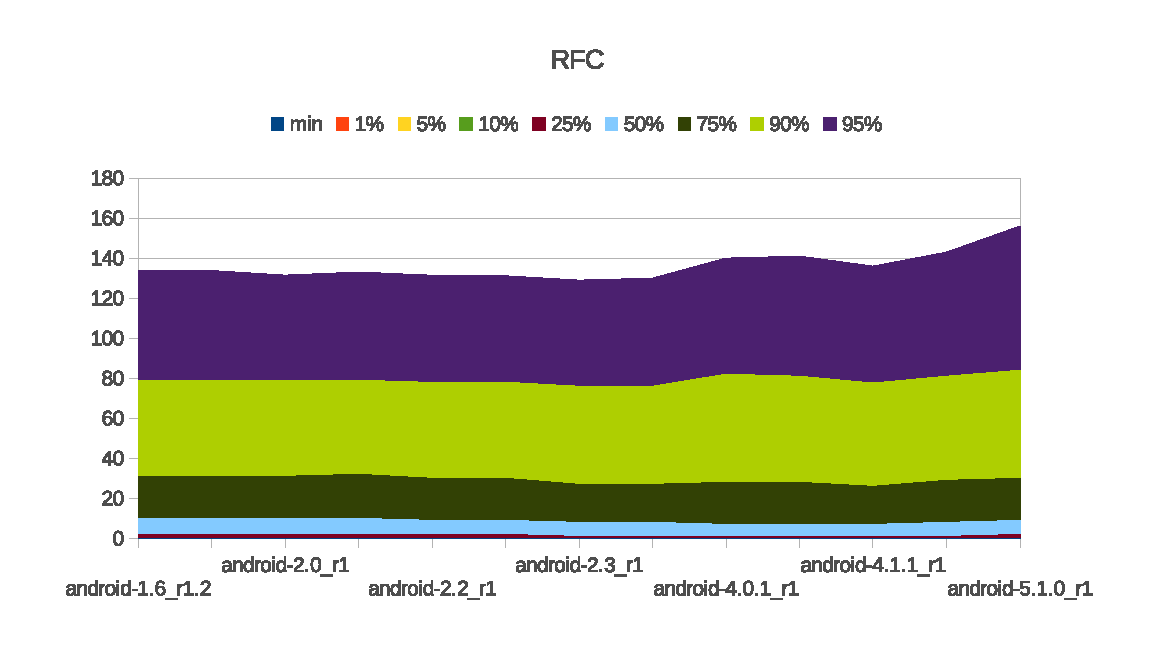
\includegraphics [keepaspectratio=true,scale=0.85]{figuras/graphs/rfc_android.eps}
\caption{Evolução da métrica RFC ao longo das versões da API}
\label{fig:rfc_android}
\end{figure}

Contribuindo para o aumento, o resultado da busca de dispositivos bluetooth é realizado de forma assíncrona na forma de mensagens utilizando \textit{intents} (vide Capítulo~\ref{cap:android-os}), então mais um método é criado dentro de um \textit{receiver} (que pode ser a própria classe estendendo \textit{BroadcastReceiver}) para receber essa mensagem, aumentando um pouco o valor de RFC. Uma comunicação síncrona hipotética com uma chamada estática direta como \textit{BluetoothAdapter.discoverNearDevices()} retornando uma lista seria em teoria uma forma muito mais simples de ser utilizada, porém perderia a proteção do encapsulamento e deixaria de utilizar o comportamento em escopo de objeto para usar em escopo de classe, e também se perderia o maior controle sobre a própria busca que a API dá ao usuário com os métodos adicionais. Além disso, o encapsulamento de serviço dos sistema é um controle adicional que permite que o mesmo escalone melhor a utilização de recursos que necessitem de exclusão mútua. Por exemplo, um acesso direto a câmera dificultaria o sistema de dar acesso a 1 cliente de cada vez, pois afinal, o usuário não consegue usar a câmera, por exemplo, em dois aplicativos simultaneamente.

Comunicações assíncronas são muito usadas ao longo de todo o sistema para utilização de recursos, e então é necessário ter uma forma de receber mensagens de aplicativos e do sistema, o que é feito com a classe \textit{BroadcastReceiver} e implementando métodos específicos da mesma. Mesmo fora do contexto Android, comunicações assíncronas tendem a criar métodos adicionais de comunicação, como é visto no padrão \textit{Observer}, que se assemelha muito a essa comunicação por \textit{Intents}. A Figura~\ref{fig:rfc_android} demonstra que essa métrica não teve variação grande ao longo das versões do Android, tendendo inclusive a um leve aumento nas ultimas versões, demonstrando que os valores altos apresentados são mesmo uma característica da arquitetura do sistema. 

\begin{table}[!htb]
\scalefont{.7}
\begin{tabular}{|l|l|l|l|l|l|l|l|l|l|l|l|}
\hline
app&min&1\%&5\%&10\%&25\%&50\%&75\%&90\%&95\%&99\%&max\\
\hline
Launcher2&0&0&1&1&3.75&12.5&37.25&84.4&178.75&850.719999999999&1061\\
\hline
Settings&0&0&0&0&3&10&31&69&112&229.2&596\\
\hline
Camera2&0&0&0&0&1&6&22&65&113&352.199999999998&752\\
\hline
Bluetooth&0&0&0&2&8&25&68.75&131.3&205.6&468.34&658\\
\hline
VoiceDialer&2&2&2&2&6&14&37&59.4&87.8999999999999&137.58&150\\
\hline
QuickSearchBox&0&0&1&1&3&8&19&30&57.3&115.12&213\\
\hline
Calculator&1&1&1&1&6&8&13&42.8&62.4&78.08&82\\
\hline
Mms&0&0&0&0&2&10&30.5&76.6&122&247.36&788\\
\hline
ManagedProvisioning&1&1&1.85&2&2.25&7.5&49.5&66.4&80.2&93.3&97\\
\hline
SoundRecorder&2&2.84&6.2&10.4&23&28&94&130.6&142.8&152.56&155\\
\hline
Terminal&0&0.15&0.75&1&3&13&47.5&52.5&56.5&64.9&67\\
\hline
PackageInstaller&0&0.17&0.85&2.4&3&10.5&26&62.5000000000001&128&155.2&162\\
\hline
SpareParts&1&1.6&4&7.00000000000001&16&31&46&55&58&60.4&61\\
\hline
Tag&1&1.14&1.7&2.4&4&9&16&20.2&25.5&33.9&36\\
\hline
CertInstaller&1&1&1&1&3.5&6&14.5&86&109.5&128.3&133\\
\hline
KeyChain&0&0.17&0.85&1.7&4&9.5&13.75&21.1&26.3&27.66&28\\
\hline
Dialer&0&0&0&1&3&8.5&25&66.4&113.1&250.74&321\\
\hline
Browser&0&0&1&1&3.25&13&36.75&78.6&124.35&328.89&795\\
\hline
PhoneCommon&0&0.17&0.85&1&3&5.5&9&30.8&43.95&52.79&55\\
\hline
InCallUI&0&0&0&0&1&8&28.25&82.5&120.25&297.349999999999&434\\
\hline
CellBroadcastReceiver&1&1&1&2&5&15.5&26&33.4&54.8&75.63&84\\
\hline
OneTimeInitializer&2&2.18&2.9&3.8&6.5&11&15.5&18.2&19.1&19.82&20\\
\hline
LegacyCamera&0&0&0&0.200000000000003&3&11&38&77.6&139.6&400.76&742\\
\hline
Gallery2&0&0&0&0&3&12&33.75&77.7&110&312.14&595\\
\hline
BasicSmsReceiver&7&7.03&7.15&7.3&7.75&12.5&24.75&38.7&43.35&47.07&48\\
\hline
MusicFX&1&1&1&1.5&2.75&5.5&35.25&125&147.5&194.3&206\\
\hline
TvSettings&0&0&1&1&3&14&41&76.9&107.65&191.599999999999&775\\
\hline
Stk&1&1.16&1.8&2.6&6&18&45&125.6&179.2&304.64&336\\
\hline
UnifiedEmail&0&0&0&1&3&9&25&59&114.5&356.8&1012\\
\hline
Launcher3&0&0&0&0&2&9&31&77.8&144.6&515.640000000001&1407\\
\hline
Music&0&0&0&1&2&6.5&19.75&45.6000000000001&94.9999999999999&155.5&192\\
\hline
Camera&0&0&0&1&2&10&33&80&128.5&307.27&921\\
\hline
Email&0&0&0&1&2.5&9&28&60&93.1999999999999&192.22&399\\
\hline
Nfc&0&0&0&1&3&16&37&93.8&155&263.44&306\\
\hline
Gallery&0&0.87&1&1&4&17&31.5&68.3&118.7&224.66&296\\
\hline
ContactsCommon&0&0&0&1&3&9&22&60&105.5&199.4&271\\
\hline
Contacts&0&0&0&1&3&8.5&23&59&96.25&253.46&463\\
\hline
DeskClock&0&0&0&1&4.75&21&50.25&121.3&151.35&230.25&691\\
\hline
FMRadio&0&0&0&0&0&0.5&18.25&75.4&105.85&277.05&414\\
\hline
\end{tabular}
\newline
\begin{tabular}{|l|l|l|l|l|l|l|l|l|l|l|l|}
\hline
HTMLViewer&1&1.06&1.3&1.6&2.5&4&4.5&4.8&4.9&4.98&5\\
\hline
Calendar&0&0&0&1&4&13&37.5&109.6&160&422.799999999998&1291\\
\hline
Exchange&0&0&0&1&4&14&37.75&72.1&107.55&162.05&224\\
\hline
\end{tabular}

\scalefont{.7}
\caption{Percentis para a métrica \textit{Response For a Class} nos aplicativos nativos}
\label{tab:rfc_apps}
\end{table}

Alto valor de profundidade de árvore de herança em uma classe pode auxiliar no aumento da métrica RFC, uma vez que todos os comportamentos são herdados. Entretanto não é uma correlação direta significativa entre as duas, visto que a profundidade de herança raramente é alta para o sistema Android, como será discutido nas seções seguintes. Embora valor alto de DIT possa significar maior valor de RFC, valores muito altos de RFC tendem a indicar mais a falta de coesão e alto acoplamento, aumentando assim a complexidade estrutural da classe, e não uma profundidade de herança preocupante.
%TODO rever esse parágrafo que compara com DIT

Em suma, na API do sistema, o valor de RFC pode ser considerado alto, porém justificável. Inclusive, o acoplamento entre a própria API de desenvolvimento e o aplicativos faz com que o valor dessa métrica seja alto também para aplicativos desenvolvidos para o Android. E importante lembrar que componentes do sistema se comunicam da mesma forma com outros componentes do sistema como se comunicam com aplicativos desenvolvidos para o mesmo. A Tabela~\ref{tab:rfc_apps} demonstra os valores de RFC para aplicativos nativos.

\citeonline{meirelles2013} define como bons intervalos para projetos Java valores de 0 a 9, 10 a 26, e 27 a 59, para os percentis 75, 90 e 95, respectivamente. Pode-ses perceber que os valores na análise da API obtidos neste trabalho estão bem acima desse valor, estando em seu percentil 75 um valor perto de 30, que seria no máximo regular nessa escala.

Baseando-se em todas essas observações, são considerados os seguintes intervalos:

%TODO rever intervalos
\begin{itemize}
\item Valores abaixo 31 se mostraram muito frequentes para API Android. Para os aplicativos do sistema, existe uma grande variância de valores, porém estando em sua grande maioria abaixo de 38 para o percentil 75.
\item RFC chegou a 130 em aplicativos nativos, porém no geral não alcançam o valor 85. Esse mesmo valor é o limite para a API do sistema.
\item Valores acima de 85 são valores considerados muito altos para a métrica RFC, e são pouco frequentes nos dados analisados.
\end{itemize}

Um intervalo de valores até 38 pode ser considerado bom para aplicativos, e regular no intervalo desse valor até o 85. Acima disso são considerados valores altos. Esses intervalos aqui encontrados estão mais próximos dos limites definidos por \citeonline{meirelles2013} para a Linguagem C do que para Java. Inclusive os valores aqui encontrados aqui para a API Android, essencialmente em Java, se mostram bastante semelhantes aos valores para o projeto Android como um todo, com predominância da linguagem C, encontrados por \citeonline{meirelles2013}. Essa semelhança pode levar a interpretação de que estilos semelhantes de estruturação e design são utilizados em todo o AOSP, independente da linguagem utilizada em cada módulo.

\subsection{Depth of Inheritance Tree / Number of Children}

Depth of Inheritance Tree (DIT) é uma métrica que mede a profundidade que uma classe se contra na árvore de herança. Se ela não herda nada, tem DIT igual a 0. Se herda de uma classe, a profundidade é 1, e assim por diante. 

Number of children (NOC) mede a quantidade de filhos que uma classe tem. Caso ninguém herde dela, o valor é 0, e aumenta em 1 para cada classe que a estende diretamente, ou seja, filhos de filhos não são contabilizados.

\begin{figure}[!htb]
\centering
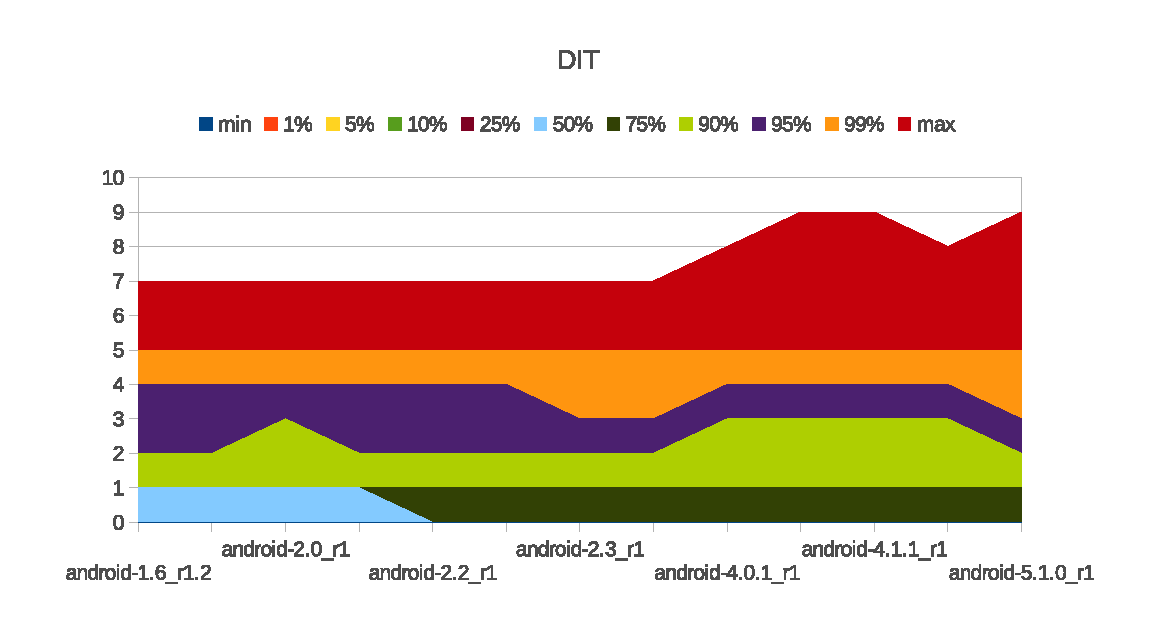
\includegraphics [keepaspectratio=true,scale=0.85]{figuras/graphs/dit_android.eps}
\caption{Evolução da métrica DIT ao longo das versões da API}
\label{fig:dit_android}
\end{figure}

\begin{figure}[!htb]
\centering
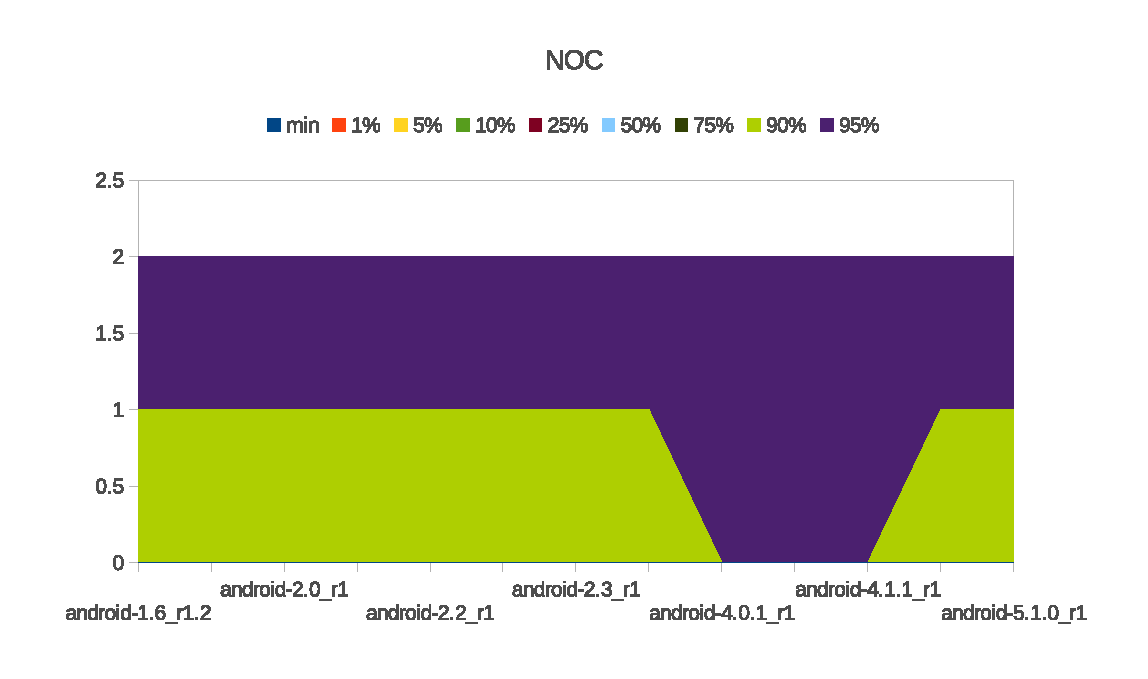
\includegraphics [keepaspectratio=true,scale=0.85]{figuras/graphs/noc_android.eps}
\caption{Evolução da métrica NOC ao longo das versões da API}
\label{fig:noc_android}
\end{figure}

DIT e NOC são métricas relativamente semelhantes por trabalhar com a árvore de herança, entretanto tem interpretações diferentes. São métricas que indicam complexidade no design, assim como a maioria das métricas OO.

As Figuras~\ref{fig:dit_android} e~\ref{fig:noc_android} demonstram o comportamento dessas métricas com a evolução do sistema. É possível perceber que são valores relativamente baixos e com variação muito pequena para as duas métricas. Para DIT podemos perceber que os valores para cada percentil varia em no máximo 1 em algumas versões e depois voltam ao valor anterior. NOC também se mantém 0 ou 1 para o percentil 90 em todas as versões.

\begin{table}[!htb]
\scalefont{.7}
\begin{tabular}{|l|l|l|l|l|l|l|l|l|l|l|l|l|}
\hline
version&classes&min&1\%&5\%&10\%&25\%&50\%&75\%&90\%&95\%&99\%&max\\
\hline
android-1.6\_r1.2&5745&0&0&0&0&0&1&1&2&4&5&7\\
\hline
android-1.6\_r1.5&5745&0&0&0&0&0&1&1&2&4&5&7\\
\hline
android-2.0\_r1&6331&0&0&0&0&0&1&1&3&4&5&7\\
\hline
android-2.1\_r2.1p2&6360&0&0&0&0&0&1&1&2&4&5&7\\
\hline
android-2.2\_r1&7352&0&0&0&0&0&0&1&2&4&5&7\\
\hline
android-2.2.3\_r2&7358&0&0&0&0&0&0&1&2&4&5&7\\
\hline
android-2.3\_r1&8093&0&0&0&0&0&0&1&2&3&5&7\\
\hline
android-2.3.7\_r1&8240&0&0&0&0&0&0&1&2&3&5&7\\
\hline
android-4.0.1\_r1&11709&0&0&0&0&0&0&1&3&4&5&8\\
\hline
android-4.0.4\_r2.1&11851&0&0&0&0&0&0&1&3&4&5&9\\
\hline
android-4.1.1\_r1&14115&0&0&0&0&0&0&1&3&4&5&9\\
\hline
android-4.3.1\_r1&15472&0&0&0&0&0&0&1&3&4&5&8\\
\hline
android-5.1.0\_r1&20129&0&0&0&0&0&0&1&2&3&5&9\\
\hline
\end{tabular}

\scalefont{.7}
\caption{Percentis para a métrica \textit{Depth of Inheritance Tree} no Android}
\label{tab:dit_android}
\end{table}

Altos valores de DIT indicam que a classe herda de várias outras recursivamente, podendo tornar seu comportamento mais imprevisível, pois não se sabe todos os seus possíveis comportamentos sem analisar as demais. Classes com alto DIT tendem a ser mais complexas por adicionar o comportamento de todas suas classes precursoras. Entretanto, por se tratar de herança, altos valores de DIT também indicam maior reuso de código fonte.

NOC também indica maior potencial de reuso em altos valores, assim como na métrica DIT. Entretanto, ela também indica a importância de uma classe e seus comportamentos no design. Um NOC alto significa que uma mudança na classe pode ter consequencias graves, pois seus métodos são utilizados em muitos filhos. Consequentemente é recomendado que classes com altos valores de NOC sejam muito bem testadas.

\begin{table}[!htb]
\scalefont{.7}
\begin{tabular}{|l|l|l|l|l|l|l|l|l|l|l|l|}
\hline
app&min&1\%&5\%&10\%&25\%&50\%&75\%&90\%&95\%&99\%&max\\
\hline
Launcher2&0&0&0&0&0&1&1&1&2&2.41&3\\
\hline
Settings&0&0&0&0&0&1&2&2&2&3&4\\
\hline
Camera2&0&0&0&0&0&0&1&1&2&3&3\\
\hline
Bluetooth&0&0&0&0&0&0&1&1&2&2&2\\
\hline
VoiceDialer&0&0&0&0&0&0&1&1&1&1&1\\
\hline
QuickSearchBox&0&0&0&0&0&1&1&2&3&5&5\\
\hline
Calculator&0&0&0&0&0&1&1&1&1&1&1\\
\hline
Mms&0&0&0&0&0&1&1&2&3&4&6\\
\hline
ManagedProvisioning&0&0&0&0&0&0&1&1&1&1&1\\
\hline
SoundRecorder&0&0&0&0&0&1&1&1&1&1&1\\
\hline
Terminal&0&0&0&0&0&0&1&1&1&1&1\\
\hline
PackageInstaller&0&0&0&0&0&1&1&1&1&1&1\\
\hline
SpareParts&1&1&1&1&1&1&1&1&1&1&1\\
\hline
Tag&0&0&0&0&0&1&1&1&1&1&1\\
\hline
CertInstaller&0&0&0&0&0.5&1&1.5&2&2&2&2\\
\hline
KeyChain&0&0.17&0.85&1&1&1&1&1&1&1&1\\
\hline
Dialer&0&0&0&0&0&0.5&1&1&1&2&2\\
\hline
Browser&0&0&0&0&0&1&1&1&2&2&2\\
\hline
PhoneCommon&0&0&0&0&0&0&1&1&1.15&1.83&2\\
\hline
InCallUI&0&0&0&0&0&0&1&1&2&2&2\\
\hline
CellBroadcastReceiver&0&0&0&0&1&1&1&1&1.45&2&2\\
\hline
OneTimeInitializer&1&1&1&1&1&1&1&1&1&1&1\\
\hline
LegacyCamera&0&0&0&0&0&0&1&2&2&3&4\\
\hline
Gallery2&0&0&0&0&0&1&1&2&2&3&4\\
\hline
BasicSmsReceiver&1&1&1&1&1&1&1&1&1&1&1\\
\hline
MusicFX&0&0&0&0&0&1&1&1.5&2.25&2.85&3\\
\hline
TvSettings&0&0&0&0&0&1&1&2&3&4&4\\
\hline
Stk&0&0&0&0&1&1&1&1&1&1&1\\
\hline
UnifiedEmail&0&0&0&0&0&1&1&2&2&3&4\\
\hline
Launcher3&0&0&0&0&0&1&1&1&2&3&3\\
\hline
Music&0&0&0&0&0&1&1&1&1&1&1\\
\hline
Camera&0&0&0&0&0&0&1&1&2&3&3\\
\hline
Email&0&0&0&0&0&1&1&1&2&2&3\\
\hline
Nfc&0&0&0&0&0&0&1&1&1&1&1\\
\hline
Gallery&0&0&0&0&0&1&1&2&2&3&3\\
\hline
ContactsCommon&0&0&0&0&0&1&1&1&2&3.10000000000002&5\\
\hline
Contacts&0&0&0&0&0&1&1&1&2&2&3\\
\hline
DeskClock&0&0&0&0&0&1&1&2&2&3&3\\
\hline
FMRadio&0&0&0&0&0&0&1&1&1&1&1\\
\hline
\end{tabular}
\newline
\begin{tabular}{|l|l|l|l|l|l|l|l|l|l|l|l|}
\hline
HTMLViewer&1&1&1&1&1&1&1&1&1&1&1\\
\hline
Calendar&0&0&0&0&0&1&1&1&2&2&2\\
\hline
Exchange&0&0&0&0&0&1&1&1&2&2&2\\
\hline
\end{tabular}

\scalefont{.7}
\caption{Percentis para a métrica \textit{Depth of Inheritance Tree} nos aplicativos nativos}
\label{tab:dit_apps}
\end{table}

A primeira observação sobre o dados das Tabela~\ref{tab:dit_android} e~\ref{tab:dit_apps} é que elas contém um número grande de zeros até o percentil 50. Como a linguagem Java representa mais de 85\% da amostra, vários desses zeros estão presentes também na linguagem Java. O que tiramos disso é que a ferramenta Analizo não contabiliza a classe Object na métrica DIT, pois caso contabilizasse o valor mínimo para o Java seria 1, visto que todo objeto Java herda de Object. Tirando esse fato não temos muitas surpresas, os valores são em geral baixos, chegando a no máximo 4 até o percentil 95 em todos as versões da API, demonstrando valores bem menores dos que os intervalos definidos por \citeonline{meirelles2013} para Java, que chegam até 2, 4 e 6 para os percentis 75, 90 e 95, respectivamente. \citeonline{oliveira2013} utiliza os mesmos intervalos para excelente, bom, e regular, respectivamente. \citeonline{ferreira2009} não define intervalos para essa métrica, mas indica um valor 2 como referência.

\begin{table}[!htb]
\scalefont{.7}
\begin{tabular}{|l|l|l|l|l|l|l|l|l|l|l|l|l|}
\hline
version&classes&min&1\%&5\%&10\%&25\%&50\%&75\%&90\%&95\%&99\%&max\\
\hline
android-1.6\_r1.2&5745&0&0&0&0&0&0&0&1&2&7&110\\
\hline
android-1.6\_r1.5&5745&0&0&0&0&0&0&0&1&2&7&110\\
\hline
android-2.0\_r1&6331&0&0&0&0&0&0&0&1&2&7&122\\
\hline
android-2.1\_r2.1p2&6360&0&0&0&0&0&0&0&1&2&7&124\\
\hline
android-2.2\_r1&7352&0&0&0&0&0&0&0&1&2&6&141\\
\hline
android-2.2.3\_r2&7358&0&0&0&0&0&0&0&1&2&6&141\\
\hline
android-2.3\_r1&8093&0&0&0&0&0&0&0&1&2&6&147\\
\hline
android-2.3.7\_r1&8240&0&0&0&0&0&0&0&1&2&6&149\\
\hline
android-4.0.1\_r1&11709&0&0&0&0&0&0&0&0&2&6&261\\
\hline
android-4.0.4\_r2.1&11851&0&0&0&0&0&0&0&0&2&6&262\\
\hline
android-4.1.1\_r1&14115&0&0&0&0&0&0&0&0&2&6&295\\
\hline
android-5.1.0\_r1&20129&0&0&0&0&0&0&0&1&2&6&398\\
\hline
\end{tabular}

\scalefont{.7}
\caption{Percentis para a métrica \textit{Number of Children} no Android}
\label{tab:noc_android}
\end{table}

A API do sistema se manteve dentro dos intervalos excelente ou bom definidos nesses outros trabalhos citados em todos os percentis analisados nesse trabalho. Os aplicativos se mantiveram dentro do intervalo excelente em todos os percentis, não ultrapassando o valor 2. Em geral, projetos mais simples tendem a fazer menos reúso de código fonte por meio de herança. Oportunidades para uma boa utilização desse recurso de orientação a objetos aparecem com o crescimento do projeto. Dessa forma, é esperado que aplicativos realmente tenham valores menores de DIT e NOC.

A Tabela~\ref{tab:noc_android} apresenta os valores da métrica NOC para o sistema Android. Percebe-se que a maioria das classes não tem filhos, tendo 0 como valor muito frequente em todas as versões da API do sistema. Da mesma forma que a métrica DIT, os valores encontrados aqui são relativamente baixos. \citeonline{meirelles2013} define para projetos Java o valor 0 como muito frequente, 1 a 2 frequente e 3 pouco frequente. O que encontramos aqui é 0 muito frequênte, 0 a 1 como frequente, e 2 como pouco frequente.

\begin{table}[!htb]
\scalefont{.7}
\begin{tabular}{|l|l|l|l|l|l|l|l|l|l|l|l|}
\hline
app&min&1\%&5\%&10\%&25\%&50\%&75\%&90\%&95\%&99\%&max\\
\hline
Launcher2&0&0&0&0&0&0&0&1&2&3.41&5\\
\hline
Settings&0&0&0&0&0&0&0&0&1&4&79\\
\hline
Camera2&0&0&0&0&0&0&0&1&2&3.39999999999998&8\\
\hline
Bluetooth&0&0&0&0&0&0&0&0&0&2.63&10\\
\hline
VoiceDialer&0&0&0&0&0&0&0&0.399999999999999&2&2&2\\
\hline
QuickSearchBox&0&0&0&0&0&0&0&2&2&3.06&4\\
\hline
Calculator&0&0&0&0&0&0&0&1&1&1&1\\
\hline
Mms&0&0&0&0&0&0&0&1&2&5&10\\
\hline
ManagedProvisioning&0&0&0&0&0&0&0&0&0.149999999999999&1.63&2\\
\hline
SoundRecorder&0&0&0&0&0&0&0&0.6&0.8&0.96&1\\
\hline
Terminal&0&0&0&0&0&0&0&0&0&0&0\\
\hline
PackageInstaller&0&0&0&0&0&0&0&0&0&0&0\\
\hline
SpareParts&0&0&0&0&0&0&0&0&0&0&0\\
\hline
Tag&0&0&0&0&0&0&0&0&2.09999999999999&6.02&7\\
\hline
CertInstaller&0&0&0&0&0&0&0&0&1.5&2.7&3\\
\hline
KeyChain&0&0&0&0&0&0&0&0&0&0&0\\
\hline
Dialer&0&0&0&0&0&0&0&1&1&2&3\\
\hline
Browser&0&0&0&0&0&0&0&1&2&2.43000000000001&4\\
\hline
PhoneCommon&0&0&0&0&0&0&0&0&0.149999999999999&0.829999999999998&1\\
\hline
InCallUI&0&0&0&0&0&0&0.25&1&2&5.69999999999999&7\\
\hline
CellBroadcastReceiver&0&0&0&0&0&0&0&0&0.449999999999999&1&1\\
\hline
OneTimeInitializer&0&0&0&0&0&0&0&0&0&0&0\\
\hline
LegacyCamera&0&0&0&0&0&0&0&1&2&3&8\\
\hline
Gallery2&0&0&0&0&0&0&0&1&2&8&17\\
\hline
BasicSmsReceiver&0&0&0&0&0&0&0&0&0&0&0\\
\hline
MusicFX&0&0&0&0&0&0&0&1&1&1&1\\
\hline
TvSettings&0&0&0&0&0&0&0&1&3&5.52999999999997&22\\
\hline
Stk&0&0&0&0&0&0&0&0&0&0&0\\
\hline
UnifiedEmail&0&0&0&0&0&0&0&1&2&5&17\\
\hline
Launcher3&0&0&0&0&0&0&0&1&2&3.48000000000002&7\\
\hline
Music&0&0&0&0&0&0&0&0&0&2.69999999999996&10\\
\hline
Camera&0&0&0&0&0&0&0&1&2&3&5\\
\hline
Email&0&0&0&0&0&0&0&1&2&4.05999999999995&9\\
\hline
Nfc&0&0&0&0&0&0&0&0.400000000000006&1&2&2\\
\hline
Gallery&0&0&0&0&0&0&0&1&2&6.38999999999999&9\\
\hline
ContactsCommon&0&0&0&0&0&0&0&0&1&4.30000000000007&15\\
\hline
Contacts&0&0&0&0&0&0&0&1&1&2.37&9\\
\hline
DeskClock&0&0&0&0&0&0&0&1&1&2&5\\
\hline
FMRadio&0&0&0&0&0&0&0&0&0&1&1\\
\hline
\end{tabular}
\newline
\begin{tabular}{|l|l|l|l|l|l|l|l|l|l|l|l|}
\hline
HTMLViewer&0&0&0&0&0&0&0&0&0&0&0\\
\hline
Calendar&0&0&0&0&0&0&0&0&1&4&8\\
\hline
Exchange&0&0&0&0&0&0&0&0&3&8.68999999999991&15\\
\hline
\end{tabular}

\scalefont{.7}
\caption{Percentis para a métrica \textit{Number of Children} nos aplicativos nativos}
\label{tab:noc_apps}
\end{table}

A tabela~\ref{tab:noc_apps} demonstra que os mesmos valores de NOC discutidos para a API do Android são válidos para os aplicativos nativos da plataforma. 

De forma geral, a complexidade da API android com relação a árvore de herança é relativamente baixa, e isso é refletido nos seus aplicativos, que pelo seu tamanho tem complexidade de herança ainda menor. Os valores de DIT e NOC são muito bons tanto para a API do sistema quanto para os aplicativo desenvolvidos para o mesmo. Vale ressaltar que ambas as métricas são calculadas apenas para linguagem OO, sendo que para C o valor é sempre 0. Como C representa cerca de 2\% das amostras, os resultados não são afetados.

Sobre árvore de herança, consideramos os seguintes intervalos para o Android:

\begin{itemize}
\item DIT até 1 e NOC igual a 0 são valores muito frequentes em todas as amostras.
\item DIT até 2 e NOC igual a 1 são valores frequentes em todas as amostras.
\item DIT até 4 e NOC igual a 2 são valores pouco frequentes para a API, mas para seus aplicativos os valores de DIT no percentil 95 permanecem no número 2.
\end{itemize}

\subsection{Lack of Cohesion in Methods}

Lack of Cohesion in Methods é uma métrica que mede coesão de uma classe. Existem algumas variações da métrica LCOM que não serão abordadas neste estudo. A variação calculada pela ferramenta Analizo e utilizada neste trabalho é a LCOM4.
%TODO colocar referencia LCOM4

LCOM4 gira em torno da ideia de que os métodos da classe estão coesos se eles utilizam os mesmos atributos dentro dessa classe. Se algum método não utiliza nada da classe, ou utiliza apenas métodos/atributos de outra classe, ele provavelmente está no lugar errado. 

A métrica então calcula quantos conjuntos de métodos relacionados existem dentro dessa classe, isto é, métodos que compartilham utilização de algum atributo ou que se referenciam. Caso existam 2 conjuntos de métodos distintos, ou seja, cada conjunto utiliza um conjunto diferente de atributos e um conjunto não utiliza nenhum método do outro, o valor de LCOM4 é 2, e significa que essa classe pode ser dividida em 2 para aumentar a coesão. O valor ideal de LCOM4 é 1, e valores maiores que isso podem indicar que a classe está com muita responsabilidade, tentando alcançar muitos propósitos distintos.

\begin{figure}[!htb]
\centering
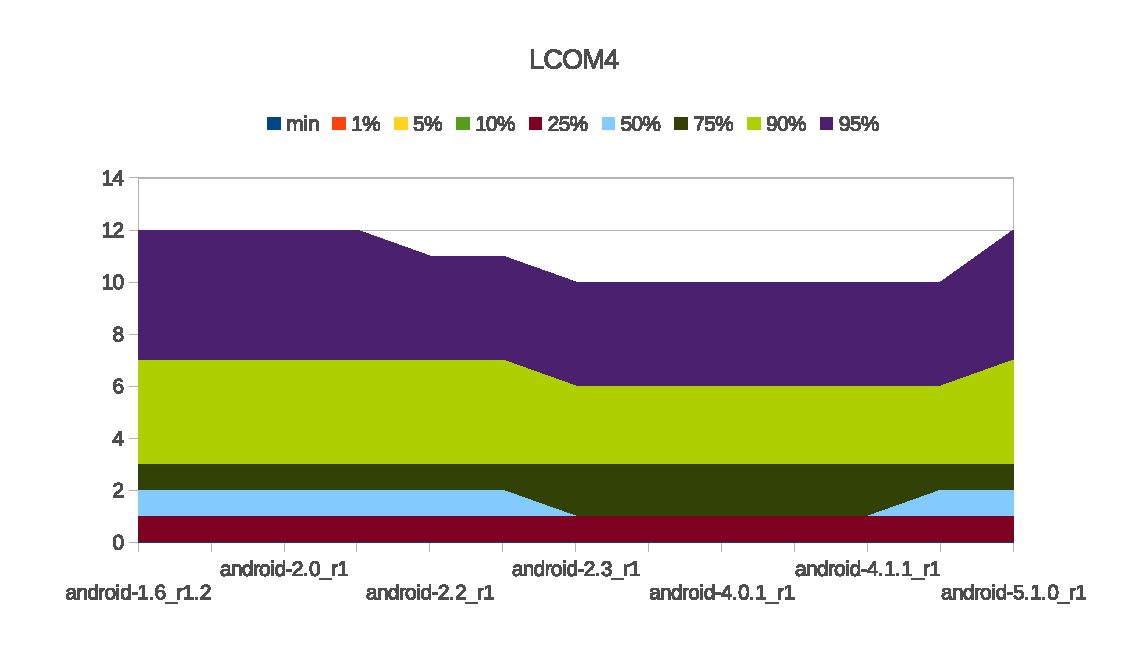
\includegraphics [keepaspectratio=true,scale=0.85]{figuras/graphs/lcom4_android.eps}
\caption{Evolução da métrica LCOM4 ao longo das versões da API}
\label{fig:lcom4_android}
\end{figure}

LCOM4 juntamente com RFC são bons indicadores da organização interna de uma classe, pois ambas as métricas dão subsídios para avaliar coesão. Essencialmente, métricas de coesão e acoplamento estão sempre relacionadas e são as métricas mais indicadas para avaliar a complexidade estrutural de uma classe. A ferramenta Analizo, por exemplo, calcula a métrica Structural Complexity (SC) como produto entre LCOM4 e CBO.

A Figura~\ref{fig:lcom4_android} apresenta a continuidade dos valores para LCOM na API do android, que, mesmo quado variam de uma versão para outra, retornam aos valores antigos, circulando acerca de um pequeno range de valores. Para o percentil 75, que representa valores muito frequentes, o gráfico demonstra uma linha reta horizontal em verde escuro que não desviou do valor 3 em nenhuma versão da API.

\begin{table}[!htb]
\scalefont{.7}
\begin{tabular}{|l|l|l|l|l|l|l|l|l|l|l|l|l|}
\hline
version&classes&min&1\%&5\%&10\%&25\%&50\%&75\%&90\%&95\%&99\%&max\\
\hline
android-1.6\_r1.2&5745&0&0&0&0&1&2&3&7&12&33&254\\
\hline
android-1.6\_r1.5&5745&0&0&0&0&1&2&3&7&12&33&254\\
\hline
android-2.0\_r1&6331&0&0&0&0&1&2&3&7&12&32&253\\
\hline
android-2.1\_r2.1p2&6360&0&0&0&0&1&2&3&7&12&33&253\\
\hline
android-2.2\_r1&7352&0&0&0&0&1&2&3&7&11&31&253\\
\hline
android-2.2.3\_r2&7358&0&0&0&0&1&2&3&7&11&31&253\\
\hline
android-2.3\_r1&8093&0&0&0&0&1&1&3&6&10&31&253\\
\hline
android-2.3.7\_r1&8240&0&0&0&0&1&1&3&6&10&31&253\\
\hline
android-4.0.1\_r1&11709&0&0&0&0&1&1&3&6&10&32.9200000000001&253\\
\hline
android-4.0.4\_r2.1&11851&0&0&0&0&1&1&3&6&10&32&253\\
\hline
android-4.1.1\_r1&14115&0&0&0&0&1&1&3&6&10&31&437\\
\hline
android-5.1.0\_r1&20129&0&0&0&0&1&2&3&7&12&89.1600000000035&1000\\
\hline
\end{tabular}

\scalefont{.7}
\caption{Percentis para a métrica \textit{Lack of Cohesion in Methods} no Android}
\label{tab:lcom4_android}
\end{table}

A Tabela~\ref{tab:lcom4_android} demonstra que em todas as versões da API Android o valor muito frequente é 3. De 3 a 7 são valores frequentes, e de 7 a 12 pouco frequentes. Valores acima de 12 não são frequentes no sistema. É possível notar, pela própria definição da métrica, que LCOM4 é limitada pelo número de métodos da classe, embora não seja diretamente relacionada. uma classe com 2 métodos não pode ter mais que 2 conjuntos distintos de métodos relacionados, então seu LCOM4 não passa de 2. Essa observação apenas quer dizer que classes pequenas tendem a ter menores valores de LCOM4.

Embora o valor ideal de LCOM4 seja 1, valores maiores que 1 não são totalmente estranhos. Muitas classes são criadas para representar alguma entidade real, e para manter seu valor semântico devem desempenhar alguns papéis distintos ao mesmo tempo. E isso é mais frequentemente visto em projetos que contém muitos dispositivos físicos acessíveis e utilizáveis no sistema. 

Em dispositivos móveis, por exemplo, tarefas de tirar foto e capturar vídeo, que são bem distintas, são reunidas na classe câmera, que representa o dispositivo físico que contempla essas funcionalidades. Essa representação de hardware em uma classe específica auxilia a manter uma maior organização no código, e mesmo que sejam tarefas distintas, resultando possivelmente em um maior valor de LCOM4, as classes ainda podem ser consideradas coesas. Fazer a separação da representação de um dispositivo físico em diversas classes pode não ser tão fácil quanto em um projeto com objetos mais ``abstratos'', que podem ser mais facilmente separados sem prejudicar o entendimento da estrutura do sistema.

\begin{table}[!htb]
\scalefont{.7}
\documentclass[a4paper]{article}
\usepackage[T1]{fontenc}
\usepackage[latin1]{inputenc}
\begin{document}
\begin{tabular}{|l|l|l|l|l|l|l|l|l|l|l|l|}
\hline
app&min&1\%&5\%&10\%&25\%&50\%&75\%&90\%&95\%&99\%&max\\
\hline
Launcher2&0&0&1&1&1&2&4&7.09999999999999&10.1&22.23&42\\
\hline
Settings&0&0&0&0&1&1&3&5&6&10.8&44\\
\hline
Camera2&0&0&0&0&1&1&3&7&11&22&135\\
\hline
Bluetooth&0&0&0&1&1&2&3&8&10.15&21.52&27\\
\hline
VoiceDialer&1&1&1&1&1&1&2&3.2&4&4&4\\
\hline
QuickSearchBox&0&0&1&1&1&2&3&6&13&21.18&30\\
\hline
Calculator&1&1&1&1&1&1&2&5.6&6.8&7.76&8\\
\hline
Mms&0&0&0&0&1&2&3&6.60000000000002&13.9&30.46&41\\
\hline
ManagedProvisioning&1&1&1&1&1&1&2&2&2.15&3.63&4\\
\hline
SoundRecorder&1&1&1&1&1&2&2&2&2&2&2\\
\hline
Terminal&0&0.15&0.75&1&1&1&3&6.5&10.75&17.35&19\\
\hline
PackageInstaller&0&0.17&0.85&1&1&1&3&4.3&5.3&6.66&7\\
\hline
SpareParts&1&1&1&1&1&1&1&1&1&1&1\\
\hline
Tag&1&1&1&1&1&2&3&3.6&4&4&4\\
\hline
CertInstaller&1&1&1&1&1&1&2&2&2&2&2\\
\hline
KeyChain&0&0.17&0.85&1&1&1&2&3.3&4.3&5.66&6\\
\hline
Dialer&0&0&0&1&1&2&3&6&9&15.87&28\\
\hline
Browser&0&0&1&1&1&2&4&6&9&32.8700000000001&54\\
\hline
PhoneCommon&0&0.17&0.85&1&1&1.5&2&3.9&6&6&6\\
\hline
InCallUI&0&0&0&0&1&2&4&6&8&14.95&25\\
\hline
CellBroadcastReceiver&1&1&1&1&1&2&3&3.9&4.45&6.38&7\\
\hline
OneTimeInitializer&1&1.01&1.05&1.1&1.25&1.5&1.75&1.9&1.95&1.99&2\\
\hline
LegacyCamera&0&0&0&0.200000000000003&1&2&3&6&7.39999999999998&22.52&47\\
\hline
Gallery2&0&0&0&0&1&2&3&6&9&17.0699999999999&38\\
\hline
BasicSmsReceiver&1&1&1&1&1&1&1.25&1.7&1.85&1.97&2\\
\hline
MusicFX&1&1&1&1&1&1&3&3.5&4&4&4\\
\hline
TvSettings&0&0&1&1&1&1&2&4&6&7.52999999999997&9\\
\hline
Stk&1&1&1&1&1&1&2&3&3.4&4.68&5\\
\hline
UnifiedEmail&0&0&0&1&1&2&3&6&10.5&25.5999999999999&76\\
\hline
Launcher3&0&0&0&0&1&2&4&7&11&33.8400000000001&51\\
\hline
Music&0&0&0&1&1&2&5&15.7&19.75&45.08&48\\
\hline
Camera&0&0&0&1&1&2&3&6&13&39.8600000000001&65\\
\hline
Email&0&0&0&1&1&2&3&7&13&46.02&144\\
\hline
Nfc&0&0&0&1&1&1&3&9.40000000000001&18&25.48&29\\
\hline
Gallery&0&0.87&1&1&1&1.5&3.25&6&9&17.52&21\\
\hline
ContactsCommon&0&0&0&1&1&2&3&6&7.5&17.1&77\\
\hline
Contacts&0&0&0&1&1&2&4&6&8&15.11&21\\
\hline
DeskClock&0&0&0&1&1&2&3&5&5.05&11.24&24\\
\hline
FMRadio&0&0&0&0&0&0.5&2&6&16.85&35.53&43\\
\hline
\end{tabular}
\newline
\begin{tabular}{|l|l|l|l|l|l|l|l|l|l|l|l|}
\hline
HTMLViewer&1&1&1&1&1&1&1.5&1.8&1.9&1.98&2\\
\hline
Calendar&0&0&0&1&1&2&3&5&6.29999999999998&31.3199999999998&51\\
\hline
Exchange&0&0&0&1&1&2&3&6&12&21.3499999999999&32\\
\hline
\end{tabular}
\end{document}

\scalefont{.7}
\caption{Percentis para a métrica \textit{Lack of Cohesion in Methods} nos aplicativos nativos}
\label{tab:lcom4_apps}
\end{table}

\citeonline{meirelles2013} define para projetos Java intervalos de 0 a 3, 4 a 7, e 8 a 12 para os percentis 75, 90 e 95, respectivamente. Os resultados encontrados aqui acompanharam muito bem esses intervalos.

LCOM4 também contabiliza classes de modelo, e no caso do Java, os \textit{getters} e \textit{setters} acarretam no aumento do valor do resultado da métrica\cite{meirelles2013}. Classes de modelo tem maior representatividade estatística em projetos menores, o que ajuda um pouco a justificar o aumento da métrica para aplicativos do sistema, como pode ser visto na Tabela~\ref{tab:lcom4_apps}. Os intervalos 0 a 4, 4 a 7, e 7 a 12 são válidos para a grande maioria dos aplicativos. Os resultados são muito parecidos com os valores para a API, sendo que a métrica só aumenta em 1 no percentil 75.

\subsection{Coupling Between Objects}

Coupling Between Objects mede o nível de acoplamento de uma classe através do número de outras classes que estão conectadas a ela de alguma forma, seja por chamada de método, uso de algum atributo/constante, uso como tipo de retorno de método, herança... Basicamente qualquer tipo de referencia. Essa verificação de referencia é feita por conexões de entrada e de saida, isto é, o valor CBO de uma classe A incrementa se uma outra classe B referencia A ou se A referencia B. Caso A referencie B, e B referencie A, numa relação bidirecional, essa relação só é contabilizada uma única vez. 

Valores menores indicam uma classe menos acoplada, e são preferíveis. Uma vez que a métrica representa uma contagem, ela não tem limite de valores, e pode ser tão grande quanto o tamanho do projeto permitir, fazendo com que projetos maiores tenham, em geral, maiores valores dessa métrica. 

\begin{table}[!htb]
\scalefont{.7}
\begin{tabular}{|l|l|l|l|l|l|l|l|l|l|l|l|l|}
\hline
version&classes&min&1\%&5\%&10\%&25\%&50\%&75\%&90\%&95\%&99\%&max\\
\hline
android-1.6\_r1.2&5745&27&89&156&312&745&1360&2023&2209&2256&2360&2394\\
\hline
android-1.6\_r1.5&5745&27&89&156&312&745&1360&2023&2209&2256&2360&2394\\
\hline
android-2.0\_r1&6331&26&90&170.5&362&788&1487&2191&2439&2478&2587&2626\\
\hline
android-2.1\_r2.1p2&6360&26&90&171&363&790.75&1502&2211&2460&2497&2604&2642\\
\hline
android-2.2\_r1&7352&26&90&193.55&453&880&1593&2396&2936&3018&3144&3185\\
\hline
android-2.2.3\_r2&7358&26&90&193.85&453&880&1595&2394&2938&3020&3146&3187\\
\hline
android-2.3\_r1&8093&7&105.92&349&536&991&1758&2676&3279.8&3361&3512&3531\\
\hline
android-2.3.7\_r1&8240&7&107&349.95&540&1007&1786&2701.25&3320&3418&3572.61&3592\\
\hline
android-4.0.1\_r1&11709&12&154&448&715&1490&2690&4041&4712&4823&5038.92&5069\\
\hline
android-4.0.4\_r2.1&11851&12&155.5&449&721&1517&2706&4095.5&4746&4873&5075&5115\\
\hline
android-4.1.1\_r1&14115&4&121.28&538.6&833&1942&3360&4896.5&5424&5665&5840&5889\\
\hline
android-4.3.1\_r1&15472&0&129&570&920&2054&3606.5&5272&6092&6316&6507&6570\\
\hline
android-5.1.0\_r1&20129&0&2&44&103&254&934&2535&4224&4505&4788&4850\\
\hline
\end{tabular}

\scalefont{.7}
\caption{Percentis para a métrica \textit{Coupling Between Objects} no Android}
\label{tab:cbo_android}
\end{table}

\begin{table}[!htb]
\scalefont{.7}
\documentclass[a4paper]{article}
\usepackage[T1]{fontenc}
\usepackage[latin1]{inputenc}
\begin{document}
\begin{tabular}{|l|l|l|l|l|l|l|l|l|l|l|l|}
\hline
app&min&1\%&5\%&10\%&25\%&50\%&75\%&90\%&95\%&99\%&max\\
\hline
Launcher2&0&1&5.95&42.9&53&74&86&90&93&95&95\\
\hline
Settings&2&8&22&39&92&181&226&265&275&292&294\\
\hline
Camera2&1&2&28&38&89&125&173&194&194&195&195\\
\hline
Bluetooth&2&3&11&18.7&32&64&98.75&116&119.3&125&125\\
\hline
VoiceDialer&2&2&2&2&2&4&4&5&5&5&5\\
\hline
QuickSearchBox&1&1.94&5.4&10&36&50&56&61&64&67&68\\
\hline
Calculator&3&3.08&3.4&3.8&4&5&5&5&5&5&5\\
\hline
Mms&0&2.08&21.1&35&48&89&131&135&138&143&143\\
\hline
ManagedProvisioning&1&1&2.7&7.5&10&11.5&17&19&19&19&19\\
\hline
SoundRecorder&1&1&1&1&1&1&4&4&4&4&4\\
\hline
Terminal&1&1&1&2.5&4&4.5&8&8.5&9&9&9\\
\hline
PackageInstaller&0&0.17&0.85&2.4&4.25&6&6.75&9&9&9&9\\
\hline
SpareParts&0&0&0&0&0&0&0&0&0&0&0\\
\hline
Tag&1&1&1&1&2&2&4&4.6&5.3&5.86&6\\
\hline
CertInstaller&3&3.1&3.5&4&4&4&4&4&4&4&4\\
\hline
KeyChain&1&1.17&1.85&2.7&3&4&5.75&6&6&6&6\\
\hline
Dialer&6&7&24&27&34&65&81&95.7&98&100.87&102\\
\hline
Browser&0&1.57&9&21&50.5&91&115&124&129&134.43&135\\
\hline
PhoneCommon&0&0.17&0.85&1&2&5&6&6&6&6&6\\
\hline
InCallUI&0&0.300000000000001&5.75&6&20&33&38&42&50&50&50\\
\hline
CellBroadcastReceiver&0&0.31&1.55&5&5&6&6&8&8&8&8\\
\hline
OneTimeInitializer&0&0&0&0&0&0&0&0&0&0&0\\
\hline
LegacyCamera&0&18&19&21&44&87&118&125.8&126&127&127\\
\hline
Gallery2&0&3&16&24.3&119&253&367.75&445&462&478&478\\
\hline
BasicSmsReceiver&0&0&0&0&0&0&0.25&0.7&0.85&0.97&1\\
\hline
MusicFX&0&0.45&2.25&3&4&4&6&6.5&7&7&7\\
\hline
TvSettings&3&4.47&14&18&50&99&141&169&180.1&186&186\\
\hline
Stk&0&0&0&0&3&3&3&3.4&4&4&4\\
\hline
UnifiedEmail&0&9&17&70&155&230&310&350&374&381&381\\
\hline
Launcher3&1&9.56&39.6&55.2&75&112&137&161&167&176.48&177\\
\hline
Music&1&1.73&2.65&4.3&9&17&24.5&29&29&29&29\\
\hline
Camera&0&18&19&22.1&51&94&133.25&148&148&149&149\\
\hline
Email&0&1&4&10&32&76&116&128.2&134&136&136\\
\hline
Nfc&1&2&11.8&15&27&59&82&101&103&103&103\\
\hline
Gallery&0&0.87&8&9&11&26&33.25&40.6&45&47&47\\
\hline
ContactsCommon&0&0&4&8&33&54&70.5&84&88&89&89\\
\hline
Contacts&2&2&8&22&45.25&70&99&108.7&110.85&114&114\\
\hline
DeskClock&0&0&4&16&20&33&48&61&64.05&66&66\\
\hline
FMRadio&10&10&10&10&10&20.5&33&38&40&41&41\\
\hline
\end{tabular}
\newline
\begin{tabular}{|l|l|l|l|l|l|l|l|l|l|l|l|}
\hline
HTMLViewer&0&0&0&0&0&0&0.5&0.8&0.9&0.98&1\\
\hline
Calendar&0&0.28&15.7&21.2&31&55&78&95&99&102.86&103\\
\hline
Exchange&0&1.33&8.6&10.3&16&40&52.75&61&62&63&63\\
\hline
\end{tabular}
\end{document}

\scalefont{.7}
\caption{Percentis para a métrica \textit{Coupling Between Objects} nos aplicativos nativos}
\label{tab:cbo_apps}
\end{table}

As Tabelas~\ref{tab:cbo_android} e~\ref{tab:cbo_apps} demonstram que os valores encontrados para essas métricas na API e nos aplicativos são absurdamente grandes. Não foi encontrado um motivo para tal, podendo então haver algum tipo de problema na ferramenta de captura. O estudo conduzido por \citeonline{meirelles2013} utiliza a mesma ferramenta e não chegou a esses valores aqui encontrados em nenhum projeto, nem mesmo na análise do código fonte completo do sistema Android. Por não conseguirmos identificar exatamente o motivo dessa discrepância de valores, serão consideradas as métricas ACC e COF para acoplamento.

\subsection{Afferent Connections per Class}

Afferent Connections per Class mede o nível de acoplamento de uma classe através do número de outras classes que fazem referencia a ela, por meio da utilização de algum método ou atributo. Apenas as conexões de entrada são contabilizadas, então, diferente de CBO que faz uma contagem bidirecinal, ACC só contabiliza a quantidade de classes clientes de uma classe A qualquer, ou seja, que referenciam A, não importando quantas classes A referencia.

Uma classe com altos valores de ACC é utilizada em muitas outras. A interpretação dessa métrica é semelhante a métrica NOC no que diz respeito a impacto de mudanças. Ter muitas classes clientes indica que é necessário um maior cuidado ao realizar edições nessa classe, uma vez que impactos dessas modificações podem ocorrer em um número de classes tão grande quanto o valor de ACC.

De forma geral, deseja-se ter classes tão independentes quanto possível, levando o valor de ACC para baixo.

\begin{table}[!htb]
\scalefont{.7}
\begin{tabular}{|l|l|l|l|l|l|l|l|l|l|l|l|l|}
\hline
version&classes&min&1\%&5\%&10\%&25\%&50\%&75\%&90\%&95\%&99\%&max\\
\hline
android-1.6\_r1.2&5745&0&0&0&0&0&0&3&12&26&137&1820\\
\hline
android-1.6\_r1.5&5745&0&0&0&0&0&0&3&12&26&137&1820\\
\hline
android-2.0\_r1&6331&0&0&0&0&0&0&3&11&25&139&1953\\
\hline
android-2.1\_r2.1p2&6360&0&0&0&0&0&0&3&11&25&139.41&1970\\
\hline
android-2.2\_r1&7352&0&0&0&0&0&0&3&12&25.45&132.98&2027\\
\hline
android-2.2.3\_r2&7358&0&0&0&0&0&0&3&12&26&132.86&2028\\
\hline
android-2.3\_r1&8093&0&0&0&0&0&0&3&11&25&114.08&2052\\
\hline
android-2.3.7\_r1&8240&0&0&0&0&0&0&3&11&25&115.22&2070\\
\hline
android-4.0.1\_r1&11709&0&0&0&0&0&0&3&11&24&122&2681\\
\hline
android-4.0.4\_r2.1&11851&0&0&0&0&0&0&3&11&24&121.5&2711\\
\hline
android-4.1.1\_r1&14115&0&0&0&0&0&0&3&11&24&117.86&2965\\
\hline
android-4.3.1\_r1&15472&0&0&0&0&0&0&3&12&25&121&3789\\
\hline
android-5.1.0\_r1&20129&0&0&0&0&0&0&3&11&22&99.72&4180\\
\hline
\end{tabular}

\scalefont{.7}
\caption{Percentis para a métrica \textit{Afferent Connections per Class} no Android}
\label{tab:acc_android}
\end{table}

Dentro do escopo de um projeto, pela própria definição da métrica, o valor limite para ACC é o próprio número de classes. Embora o valor seja limitado pelo número de classes, não é possível perceber uma relação direta entre o crescimento do número de classes e o valor de ACC, sendo que essa métrica é mais relacionada à forma como o sistema foi pensado e desenhado do que com o seu tamanho. 

\begin{figure}[!htb]
\centering
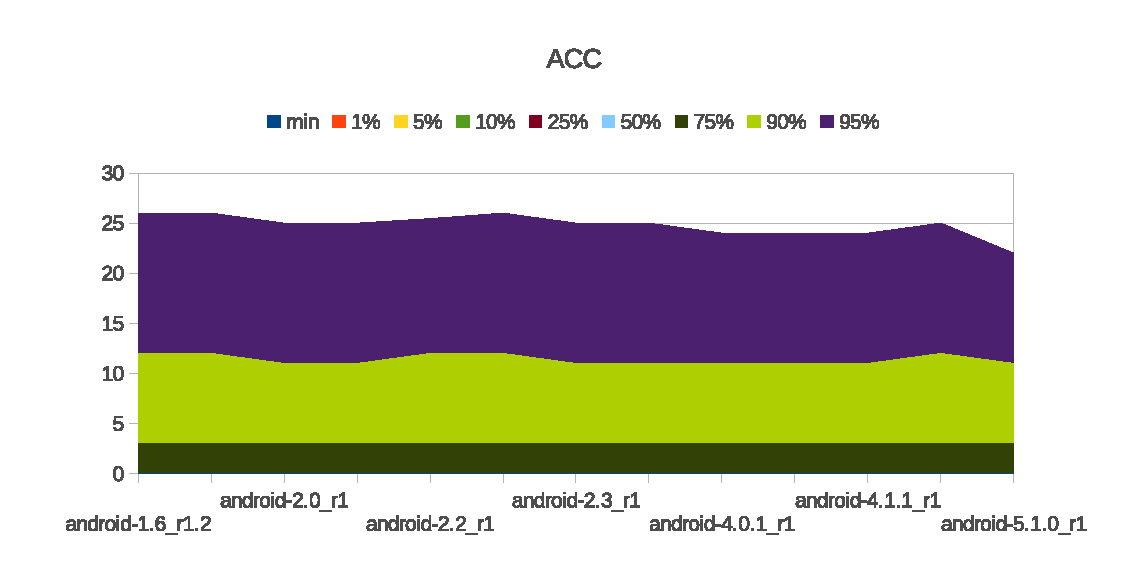
\includegraphics [keepaspectratio=true,scale=0.85]{figuras/graphs/acc_android.eps}
\caption{Evolução da métrica ACC ao longo das versões da API}
\label{fig:acc_android}
\end{figure}

A Figura~\ref{fig:acc_android} e a Tabela~\ref{tab:acc_android} demonstram que os valores da métrica ACC para os percentis 75, 90 e 95 não passam de 3, 12 e 26, respectivamente. \citeonline{oliveira2013} define os intervalos 0 a 2, 2 a 7, e 7 a 15 como excelente, bom e regular para os valores dessa métrica. \citeonline{meirelles2013} define como referencia para java os intervalos 0 a 1, 1 a 5, e 5 a 12 para os percentis 75, 90 e 95, respectivamente.

Os valores encontrados para o Android estão altos quando comparados com esses estudos, e portanto estes não são bem aplicáveis à API do Android, que, como podemos ver na Figura~\ref{fig:acc_android}, contém valores que não parecem ter tendência clara de reduzir para os intervalos considerados bons. A variância dentre as versões da API aqui analisadas é muito baixa, uma vez que quase os mesmos valores podem ser vistos ao longo das versões. Como os intervalos encontrados são constantes ao longo das versões, parecem refletir o design do sistema e podem ser utilizados como referência.

\begin{table}[!htb]
\scalefont{.7}
\begin{tabular}{|l|l|l|l|l|l|l|l|l|l|l|l|l|}
\hline
app&classes&min&1\%&5\%&10\%&25\%&50\%&75\%&90\%&95\%&99\%&max\\
\hline
Launcher2&161&0&0&0&0&0&2&5.25&17.1&26.1&92.38&110\\
\hline
Settings&722&0&0&0&0&0&0&2&6&10&26.6&307\\
\hline
Camera2&462&0&0&0&0&0&0&3&10&18&43.6&122\\
\hline
Bluetooth&239&0&0&0&0&0&1&5&16&31&81.5&169\\
\hline
QuickSearchBox&196&0&0&0&0&0&0&2&6&9&24.56&54\\
\hline
Calculator&10&0&0&0&0&0&2&2&2.4&3.2&3.84&4\\
\hline
Terminal&17&0&0&0&0&0&1&2.25&5&8.25&13.65&15\\
\hline
PackageInstaller&19&0&0&0&0&0&0.5&1&3.3&4.3&5.66&6\\
\hline
Dialer&215&0&0&0&0&0&1&3&6.7&11&16.87&35\\
\hline
Browser&259&0&0&0&0&0&1&3&8&15.15&58.16&122\\
\hline
InCallUI&117&0&0&0&0&0&1&3&6.5&10.5&25.55&93\\
\hline
LegacyCamera&214&0&0&0&0&0&2&6&11.8&16&53.4&91\\
\hline
Gallery2&895&0&0&0&0&0&1&4&11&21.35&75&150\\
\hline
BasicSmsReceiver&5&0&0&0&0&0&0&0.25&0.7&0.85&0.97&1\\
\hline
UnifiedEmail&872&0&0&0&0&0&0&3&10&16&53&160\\
\hline
Launcher3&354&0&0&0&0&0&1&4&14.8&21.8&72.24&124\\
\hline
Music&75&0&0&0&0&0&0&1&2&2.7&6.7&14\\
\hline
Camera&253&0&0&0&0&0&2&5&11.9&18.25&57.13&103\\
\hline
Email&400&0&0&0&0&0&0&1&6&18.1&40.22&201\\
\hline
Nfc&178&0&0&0&0&0&1&4&11.4&18&61.48&67\\
\hline
Gallery&89&0&0&0&0&0&1&4&8.3&13&49.13&50\\
\hline
ContactsCommon&292&0&0&0&0&0&0&1&7&15&69.4&108\\
\hline
Contacts&265&0&0&0&0&0&0&2&5&10&14.37&30\\
\hline
DeskClock&121&0&0&0&0&0&1&6&12&20&32.91&37\\
\hline
HTMLViewer&4&0&0&0&0&0&0&1&1.6&1.8&1.96&2\\
\hline
Calendar&216&0&0&0&0&0&0&4&9&18&29.44&45\\
\hline
Exchange&135&0&0&0&0&0&0&2&5&10.05&71.54&108\\
\hline
\end{tabular}

\scalefont{.7}
\caption{Percentis para a métrica \textit{Afferent Connections per Class} nos aplicativos nativos}
\label{tab:acc_apps}
\end{table}

A Tabela~\ref{tab:acc_apps} demonstra que os valores para os aplicativos do sistema também são maiores que os intervalos definidos em outros estudos. Entretanto, eles são mais parecidos com os valores encontrados dentro da própria API, mais uma vez refletindo a semelhança de aplicativos em relação a mesma, e demonstrando um certo padrão para códigos relacionados ao Android. Para a grande maioria dos aplicativos, os percentis 75, 90 e 95 não ultrapassam os valores 4, 12 e 22, respectivamente.

Consideramos então os seguintes intervalos para o Android:

\begin{itemize}
\item Para o percentil 75, ACC igual a 3 para a API e 4 para aplicativos;
\item 12 é um limite recorrente para o percentil 90 para aplicativos e para a API;
\item Para o percentil 95 em diante, aplicativos tem um valor médio menor que a API, estando com limites até 22 e 26, respectivamente.
\end{itemize}

\subsection{Coupling Factor}

Coupling Factor nada mais é que uma relativização do valor de ACC para o tamanho do projeto, sendo então um valor apenas para todo o código fonte desse projeto. ACC calcula as conexões que uma classe tem, enquanto COF soma todas essas conexões de todas as classes e divide pelo total de conexões possíveis, resultando e um valor que pode variar de 0 a 1. Caso todas as X conexões possíveis aconteçam em um software, COF para ele será X/X, que é igual a 1. O ideal então como acoplamento para um projeto qualquer é que o valor de COF esteja tão próximo de zero quanto possível, indicando que as classes são mais independentes e desacopladas.

\begin{table}[!htb]
\begin{center}
\scalefont{.7}
\begin{tabular}{|l|l|l|}
\hline
version&classes&cof\\
\hline
android-1.6\_r1.2&5745&0.0013695147\\
\hline
android-1.6\_r1.5&5745&0.001369545\\
\hline
android-2.0\_r1&6331&0.0012379467\\
\hline
android-2.1\_r2.1p2&6360&0.0012384764\\
\hline
android-2.2\_r1&7352&0.0010625123\\
\hline
android-2.2.3\_r2&7358&0.0010616483\\
\hline
android-2.3\_r1&8093&0.0009540904\\
\hline
android-2.3.7\_r1&8240&0.000937113\\
\hline
android-4.0.1\_r1&11709&0.0007400012\\
\hline
android-4.0.4\_r2.1&11851&0.0007300137\\
\hline
android-4.1.1\_r1&14115&0.0005968253\\
\hline
android-4.3.1\_r1&15472&0.0005764279\\
\hline
\end{tabular}

\scalefont{.7}
\caption{Percentis para a métrica \textit{Coupling Factor} no Android}
\label{tab:cof_android}
\end{center}
\end{table}

\begin{figure}[!htb]
\centering
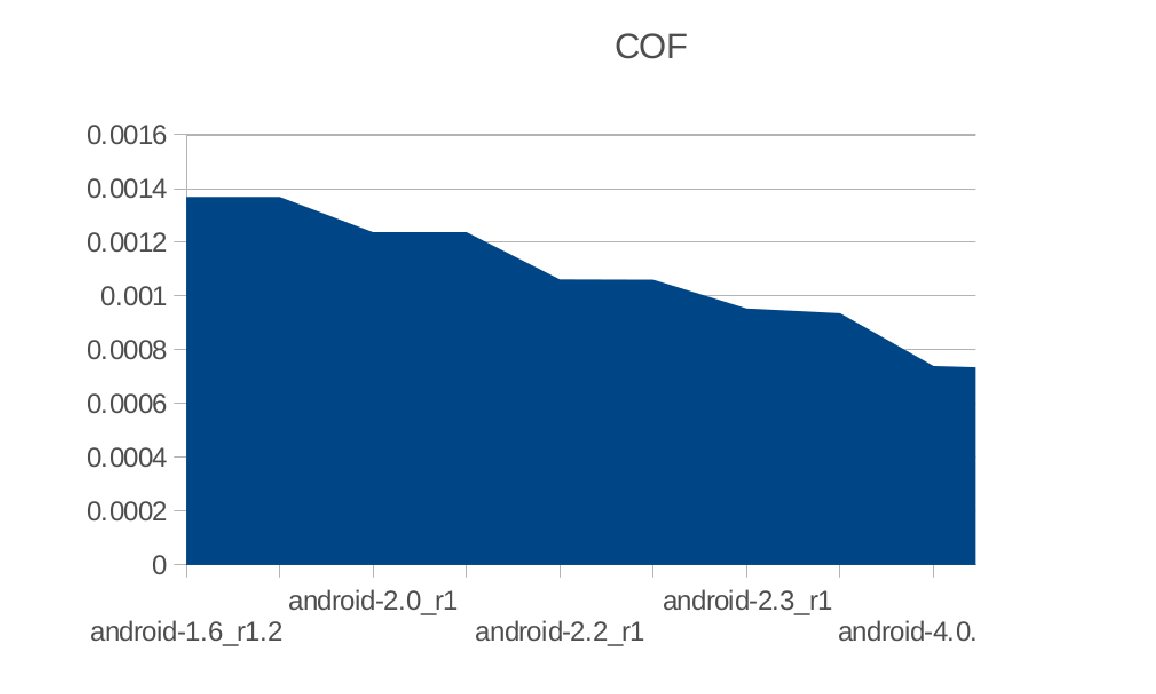
\includegraphics [keepaspectratio=true,scale=0.7]{figuras/graphs/cof_android.eps}
\caption{Evolução da métrica COF ao longo das versões da API}
\label{fig:cof_android}
\end{figure}

%TODO atualizar valores quando obtiver mais versões
%Como o denominador da expressão de cálculo dessa métrica é da ordem de O($n^2$), e o numerador O(n), n
Naturalmente o incremento no número de classes de um projeto tende a fazer com que o valor da métrica caia, embora não seja sempre inversamente proporcional a ponto de esperar que projetos distintos com números maiores de classes sempre tenham menores valores de COF, pois depende bastante do design de sua arquitetura. Para um mesmo projeto, essa relação se mostra válida como demonstra a Figura~\ref{fig:cof_android} e a Tabela~\ref{tab:cof_android}. O valor de COF para a API do Android ao longo de suas versões caiu de 0.13\% para 0.057\%. Isso se dá pelo fato de que, como demonstrado na seção anterior, o valor de ACC permanece relativamente constante enquanto o número de classes aumenta significativamente a cada versão. Essencialmente, O sistema se mostra cada vez mais desacoplado e consequentemente manutenível.

\begin{table}[!htb]
\begin{center}
\scalefont{.7}
\begin{tabular}{|l|l|l|}
\hline
app&classes&total\_cof\\
\hline
BasicSmsReceiver&5&0.0833333333\\
\hline
Calculator&10&0.1666666667\\
\hline
Calendar&216&0.014844599\\
\hline
Camera&253&0.0195566939\\
\hline
Browser&259&0.0161825476\\
\hline
Bluetooth&239&0.0259014998\\
\hline
ContactsCommon&292&0.0110795118\\
\hline
DeskClock&121&0.0343837535\\
\hline
Dialer&215&0.0119125971\\
\hline
Gallery&89&0.0432340648\\
\hline
Email&400&0.0083122379\\
\hline
Exchange&135&0.0253619122\\
\hline
HTMLViewer&4&0.3333333333\\
\hline
Music&75&0.0111069974\\
\hline
InCallUI&117&0.028035982\\
\hline
Nfc&178&0.0273497689\\
\hline
LegacyCamera&214&0.0230312694\\
\hline
Launcher2&161&0.0415487421\\
\hline
PackageInstaller&19&0.0653594771\\
\hline
QuickSearchBox&196&0.0111551679\\
\hline
Contacts&265&0.0070284595\\
\hline
Camera2&462&0.0079222861\\
\hline
Launcher3&354&0.0148564254\\
\hline
SoundRecorder&6&0.95\\
\hline
Terminal&17&0.1416666667\\
\hline
Settings&722&0.0040414548\\
\hline
Gallery2&895&0.0055753048\\
\hline
UnifiedEmail&872&0.0044023912\\
\hline
\end{tabular}

\scalefont{.7}
\caption{Percentis para a métrica \textit{Coupling Factor} nos aplicativos nativos}
\label{tab:cof_apps}
\end{center}
\end{table}

A Tabela~\ref{tab:cof_apps} apresenta os valores para os aplicativos e nela é possível perceber que o valor de COF não é sempre inversamente proporcional a quantidade de classes como já comentado, embora ele realmente tenha a tendencia a diminuir com o aumento do número de classes. Para os aplicativos, tivemos um range de 33\% para o menor dos projetos, com apenas 4 classes, e 0.4\% para um dos maiores aplicativos.

\citeonline{ferreira2009} apresenta como intervalos os valores de 0 a 0.02 (2\%) como bons , 0.02 a 0.14 (14\%) como regulares, e 0,14 em diante como valores ruins. Podemos perceber que os valores para o sistema Android estão bem abaixo desses valores, sendo considerados então excelentes valores para o fator de acoplamento. Já os aplicativos demonstraram que se mantém nos valores bons quando passam a ter por volta de 200 classes, mas quado muito pequenos se mostraram em sua maioria regulares nessa escala. 

Os intervalos aqui não são considerados em função de seus percentis, mas as seguintes observações podem ser feitas:

\begin{itemize}
\item Espera-se que o valor de COF para o sistema se mostre cada vez menor à medida que novas versões surgem;
\item Aplicativos desenvolvidos para o Android, quando muito pequenos, até poucas dezenas de classes, tendem a ficar abaixo de 10\%, e não devem ultrapassar os 14\% no valor de COF. Valores bem menores ainda podem ser obtidos e são preferíveis;
\item A medida que ganham tamanho de várias dezenas à poucas centenas de classes, os valores de COF para aplicativos não devem ultrapassar os 4\%, entretanto é recomendável que fique abaixo de 2\%. Quando chegam a várias centenas de classes, os valores devem ser menores que 1\%.
\end{itemize}

\section{Modelos de Regressão}

A partir da obtenção e analise preliminar dos dados de métricas OO nas diferentes versões do Android e de aplicativos nativos, foram feitos testes empíricos para verificar da possibilidade de utilizar esses dados em modelos de regressão polinomial. Essas tentativas tiveram como alvo a predição de um valor ideal de uma métrica para aplicativos em desenvolvimento, a partir de alguma métrica independente base, que refletisse o tamanho do projeto analisado. 

Algumas das métricas base que foram inicialmente idealizadas para relativização das métricas para diferentes tamanhos de projetos e regressão polinomial:

\begin{enumerate}
\item Número de classes, realizando uma regressão em escopo de software.
\item Número de classes por pacote, resultando em uma regressão em escopo de ``módulo''.
\item Número de métodos, realizando uma regressão em escopo de classe.
\item AMLOC, realizando uma regressão em escopo de classe.
\end{enumerate}

Não é possível idealizar esse resultado para métricas OO, mensuradas para cada classe, para entradas mais granularizadas como valores de métodos.

O objetivo era relativamente simples: desejava-se, a partir do tamanho de um projeto/módulo/classe, obter o valor ideal para uma métrica a fim de o desenvolvedor pudesse comparar com o valor real que o código possui, e então verificar se mudanças estruturais devem ser feitas. Com isso, validar então os intervalos aqui definidos na seção anterior como bons valores nesse contexto de desenvolvimento em Java para a plataforma Android.

Nenhuma das formas propostas foi realmente desenvolvida, apenas foi realizado uma discussão rápida das possibilidades com as métricas que estavam disponíveis. Métricas de tamanho foram o alvo da regressão como variáveis independentes porque seriam uma forma de abstrair os resultados para projetos de diferentes escalas.

\subsection{Regressão em escopo de software}

A primeira observação que se faz sobre a realização de regressão em escopo de software utilizando os valores da evolução da API do sistema Android é capacidade de generalização de um modelo. De forma geral, o modelo seria criado com pontos com valores de número de classes variando de 5000 a 20000 classes. Como consequência, o modelo de regressão não teria uma boa capacidade de generalização para projetos muito pequenos, como acontece com aplicativos, que possuem muitas vezes apenas algumas dezenas de classes, e são o alvo principal para utilização dessa regressão. Da mesma forma, a capacidade de predição para projetos que contenham bem mais que 20000 classes também seria prejudicada, uma vez que o modelo de regressão não veria nenhum nesse intervalo. Isso tudo assumindo que os dados obedecem um certo padrão e um funcional realmente pode ser traçado que represente o comportamento dos mesmos. 

Para que isso pudesse ser realmente feito, os dados das métricas OO devem ser relacionados com as métricas de tamanho, demonstrando seu valor como dependente do valor dessas métricas.

%TODO demonstrar graficos ACC, ACCM, LCOM4, e RFC em função do numero de classes

Como podemos ver na Figura XXXX, onde é traçado o percentil 75 em função do número de classes, as métrica ACC, LCOM4 e ACCM parecem poder ser representadas por uma linha reta horizontal, enquanto RFC tem dados muito difusos para serem representados por um polinômio. Resumidamente, para algumas métricas essa regressão parece ser promissora, isto é, um funcional realmente pode ser traçado que representa a variação dos valores das métricas com o número de classes do projeto. Entretanto, a ínfima variação para métricas importantes como ACC, LCOM4, DIT, NOC, ACCM, que são as principais métricas aqui analisadas, dá a impressão de que um valor referência se mostra tão útil quanto essa regressão, tornando-a desnecessária.

Além de poder utilizar um valor referencia sem perda de valor semântico sobre o valor ideal da métrica, uma regressão em escopo de software da forma como foi proposta, pelo número de classes, não contém, com os dados aqui obtidos, um conjunto suficiente de dados para uma boa regressão, mesmo se ela se apresentasse realmente necessária. Em suma, temos poucas amostras para realizar esse estudo. Com os valores das métricas para todos as TAGS no repositório do AOSP talvez uma regressão poderia ser melhor realizada, porém, como já comentado, os dados aqui obtidos indicam q ela seria extremamente próxima de uma linha reta horizontal para a maioria das métricas, dado o grau de independência que elas demonstram em relação ao número de classes.

Como um pequeno problema adicional para esse tipo de regressão linear com os dados aqui obtidos seria um problema de \textit{overfitting}, ou seja, um ajuste muito fino em relação aos dados. Os dados das métricas para os aplicativos se mostraram levemente diferentes para os dados da API do sistema, mesmo estando bem semelhantes, então utilizar apenas a API do sistema como insumo para o modelo de regressão resultaria em um modelo que não funciona bem para predizer valores de métricas de aplicativos. Entretanto, para os aplicativos, considerando cada um como um projeto distinto, assim como fizemos com as versões da API, as métricas são extremamente dispersas em relação ao número de classes, tornando difícil representar os dados por um polinômio para realizar a regressão. Isso se dá pela maior variância que as métricas tem nos aplicativos devido às diferenças dos propósito desses aplicativos, o que muda seu estilo de arquitetura. Assim, podemos chegar a conclusão que uma regressão por número de classes pode ser válida para diferentes versões sistemas estáveis, que tenham variações de tamanho dentro de um certo intervalo conhecido, mas não para um conjunto muito distinto de projetos.

Para realização de um modelo de regressão polinomial a nível de software, não foi encontrada ao longo deste trabalho, dadas restrições de tempo e escopo, outra métrica que representasse bem o tamanho do projeto para relativização do resultado das métricas OO, que foram selecionadas para avaliar a arquitetura no contexto do desenvolvimento para Android. 

Utilizar a quantidade de pacotes em vez da quantidade de classes teria o mesmo efeito, uma vez que as métricas OO também são independentes desse valor.
%TODO demonstrar que as métricas não dependem da quantidade de pacotes assim como não dependem da quantidade de classes (será q precisa???)

\subsection{Regressão em escopo de classe}

Como uma segunda tentativa na direção de uma regressão polinomial para aplicativos, foi verificada a possibilidade de utilizar valores das métricas para classes, em vez de utilizar todo o conjunto de classes com uma abordagem estatística de percentis, como foi comentado na seção anterior. Tentamos então avaliar o valor ideal de uma métrica para uma classe, dado alguma variável independente que represente de alguma forma seu tamanho.

Cada classe dentro de cada versão seria uma amostra para esse método, que teria então um total de mais de 100000 classes. Pensando dessa forma o problema de escala do escopo de software seria resolvido, uma vez que no próprio sistema existem classes com um range muito grande de tamanhos. Então para cada amostra utilizada com um modelo em produção, o mesmo já teria visto uma com parâmetros de tamanho semelhantes em sua criação. 

O problema nessa abordagem é que as métricas de tamanho que podem ser utilizadas também se mostraram bem independentes dos valores das métricas OO. AMLOC por exemplo, não interfere em LCOM4, pois métodos grandes podem ser bastante coesos e métodos pequenos podem não ser, dependendo mais da responsabilidade da classe. Isso faz com que a variação das métricas OO em função de AMLOC ou NOM se apresente bem difusa como mostra o gráfico da Figura XXXX.
%TODO apresentar graficos de algumas métricas em função de AMLOC, e em funcao de NOM

Em suma, os valores das métricas não são relacionados com os valores dessas métricas de tamanho, como mostra a matriz de correlação XXXX.
%TODO criar matriz de correlação

\subsection{Regressão em escopo de pacote}

Para fazer esse teste, foi separado cada pacote presente em cada versão do sistema, e utilizado como métrica de tamanho o número de classes nesse pacote. O problema encontrado foi que as métricas eram totalmente dependentes do próprio pacote analisado e seu propósito, mas independentes de seu tamanho. Isso quer dizer que 2 pacotes de 3 classes cada apresentavam valores com nenhuma relação entre si. Basicamente, o mesmo problema de independência dos dados em relação a variável de tamanho foi encontrada nessa abordagem.

O gráfico da figura XXXX demonstra a metrica XXXX para cada pacote em função dos seu número de classes. Podemos pereber que os valores tem uma grande variação que aparentemente independe do número de classes do pacote, mas sim do propósito e das responsabilidades do mesmo.

\subsection{Conclusão acerca de regressão}

As métricas OO se mostraram independentes de tamanho. Algumas análises foram feitas na seção de análise preliminar demarcando alguns valores para diferentes tamanhos do projeto quando aplicável. A grande maioria não teve variação significativa em relação a nenhuma das métricas de tamanho que foram obtidas.

Regressão nesse contexto não se mostrou um esforço válido para auxiliar desenvolvimento futuro de aplicativos. Afinal, a maioria dos valores se mostrou invariável ao longo das versões, ou com intervalos fixos. Dessa forma, utilizar esses intervalos tem tanta utilidade quanto uma regressão apresentaria. Para métricas OO, utilizar valores ou intervalos de referência é uma prática mais simples e ainda eficaz enquanto se desenvolve aplicativos, uma vez que a arquitetura do sistema é avaliada dependendo de alguns parâmetros e os intervalos de valores, como exemplificado para algumas métricas na seção anterior.
